\subsection{Standard Model W+Jets}
\label{sec:Bkg:wjet}

\indent W boson produced in conjunction with QCD jets ($W$+jets) consists our largest sub-dominate background.  $W$+jets consists of 5 percent of the total background in the SR.  However the distribution of $W$+jets is not uniform across $\RISR$.  $W$+jets can reach around 15 percent of all background in the SR bins with the largest $\RISR$.  This means the $W$+jets contribution mostly affects the signal with high stop masses because those signal samples peak at high $\RISR$. \\
\indent We estimate $W$+Jets using a 1 lepton control region defined in section \ref{sec:WCR}.  The 1 lepton $W$+jet CR is orthogonal to the 1 lepton ttbar CR and 1 lepton single top CR defined in table \ref{tab:ttbar1LepCRISR_def} and \ref{tab:singleTop1LepCR_def} .  The $W$+jets prediction is checked in a $W$+jets validation region defined in section \ref{sec:WVR} \\



\subsubsection{\Wjets\ Control Region}
\label{sec:WCR}

\begin{table}[htpb]
  \caption{Summary of the selection for the 1-lepton, $W$+jets control regions. The signal lepton is treated as a jet for the jet counting and \pt\ ordering as well as for the top reco.}
  \begin{center}
    \begin{tabular}{c|c}
      \hline \hline
                                      & CRW                \\ \hline
      Number of leptons             & 1                                          \\ \hline
      Number of jets (incl. lepton) & $\geq 4$                                     \\ \hline
      $\pt$ of jets (incl. lepton)  & (80,80,40,40) GeV                            \\ \hline
      \mindphijettwomet             & $> 0.4$                                      \\ \hline
      $\met$                        & $>250$ GeV                                   \\ \hline
      %\mtlepmet                    & $>30$,$<120$ GeV              & \multicolumn{2}{c}{$>30$,$<100$} \\ \hline
      \mtlepmet                     & ($>30, <100$ GeV) \\ \hline
      Number of $b$-jets            & $=1$                            \\ \hline
      %Number of $b$-jets           & \multicolumn{2}{c|}{$\geq 2$} & $=1$                             \\ \hline
      \mantikttwelvezero            & $<60\,$GeV         \\ \hline
      %\mtbmin                      & $>100\,$GeV                   & $>200\,$GeV & -                  \\ \hline
      %\mindrblep                   & $<1.5$                        & $>1.5$      & $>2.0$             \\ \hline
      \mindrblep                    & $>2.0$             \\ \hline \hline
    \end{tabular}
  \end{center}
  \label{tab:WJetCR}
\end{table}

$\mantikttwelvezero < 60 \gev$ ensures that no boosted tops are reconstructed.  The number of b-tagged jets ensures orthogonality with the single top CR.  The selection on $\Delta R(b_{0,1},\ell)_{\mathrm{min}}$, defined as the minimum $\Delta R$ between the two jets with the highest b-tag weight and the selected lepton, ensures the orthogonality of ttbar CR and $W$+jet CR.   \\

Data/MC comparisons in the \Wjets\ control region are shown in Fig.~\ref{fig:CRWpts}, \ref{fig:CRW}, \ref{fig:CRWMasses} and the yields in in Table~\ref{tab:CRW_yields}. The MC is normalised to \intlumi\ \ifb, and no normalisation factors are applied to any of the SM components. Only variables for which there is an extrapolation from CRW to the various SRs are shown. For SRA the extrapolation is in \met, \drbjetbjet, \mantikttwelvezero,  \mantikttwelveone, and \mantikteightzero\ while for SRB the extrapolation is in \mtbmin\, \mtbmax, and \drbjetbjet. The leading jet \pt s and the leading b-tagged jet \pt\ are shown because for these variables there is an extrapolation from CRW to SRD while the \met, \mtbmin, \HT, \htsig, \mantikteightzero, and \mantikteightone\ are shown due to the extrapolation to SRE. The signal contamination is less than 10\% for all signal points with the largest contamination coming from the pure bChino decay of stops with mass 500 GeV and LSP mass of 50 GeV where the chargino mass is assumed to be 100 GeV. No particular trends are observed in the data-MC ratios in any of the distribution. Within statistical uncertainty the data are compatible with the MC SM expectation. \\

\begin{table}[!htb]
  \centering
  \begin{tabular}{c|c}
\hline\hline
\multicolumn{2}{c}{\bf CRW (60\% purity)} \\ \hline 
Z & 1.99 $\pm$ 0.45 \\
dibosons & 9.85 $\pm$ 1.76 \\
ttbar & 128.42 $\pm$ 3.82 \\
singleTop & 51.14 $\pm$ 3.37 \\
ttV & 1.07 $\pm$ 0.16 \\
W & 288.12 $\pm$ 8.86 \\
\hline
Total MC & 480.58 $\pm$ 10.38 \\
Data & 531.00 $\pm$ 23.04 \\
 \hline
SF & 1.17 $\pm$ 0.10 \\
\hline\hline
\end{tabular}

  \caption{Yields in the CRW in \intlumi\ \ifb\ of data.  }
  \label{tab:CRW_yields}
\end{table}

\begin{figure}[!htb]
  \centering
  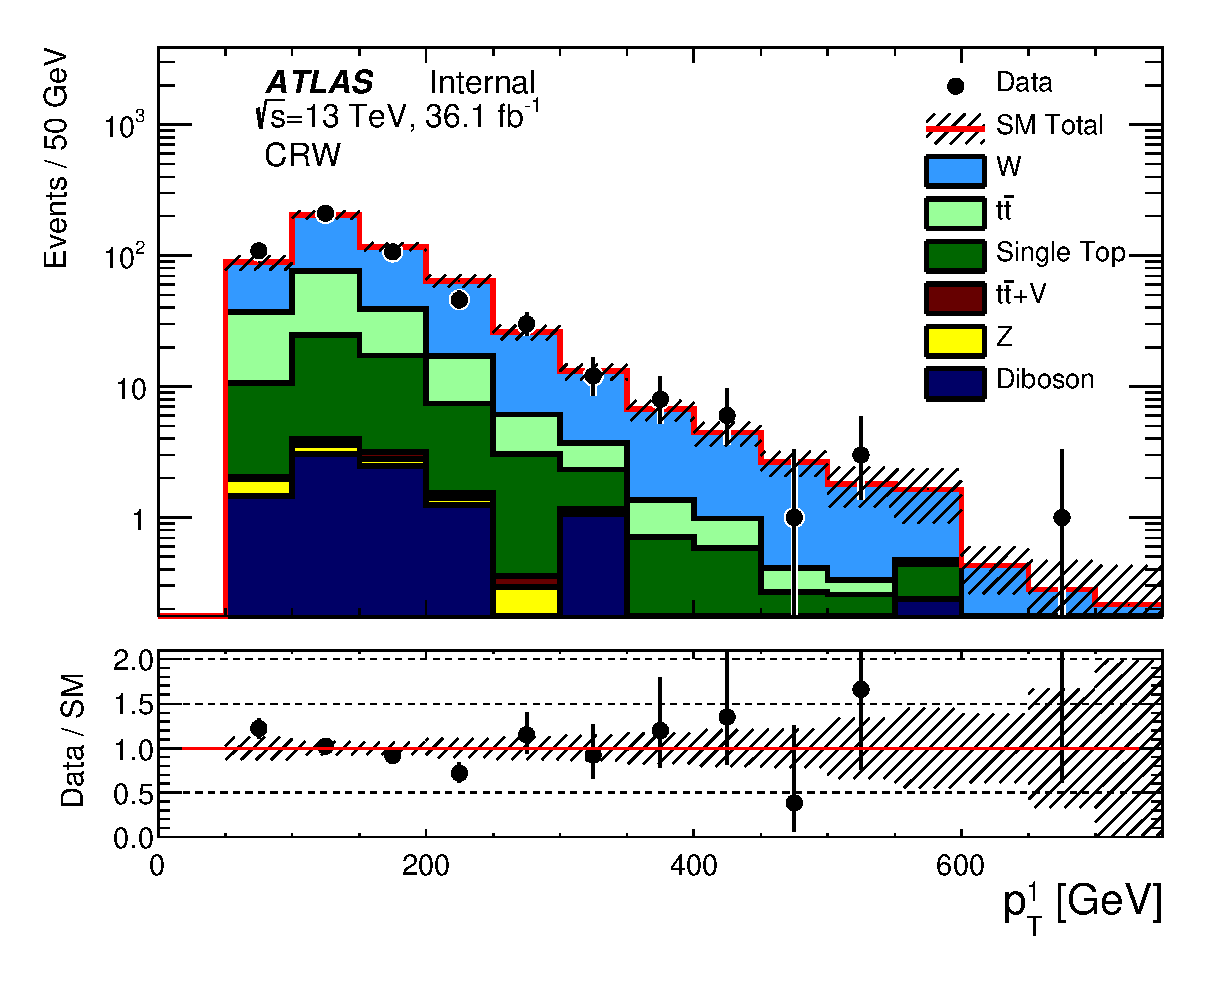
\includegraphics[width=0.45\textwidth]{figures/wJets/postfit/JetPt_1__CRW_log.eps}
  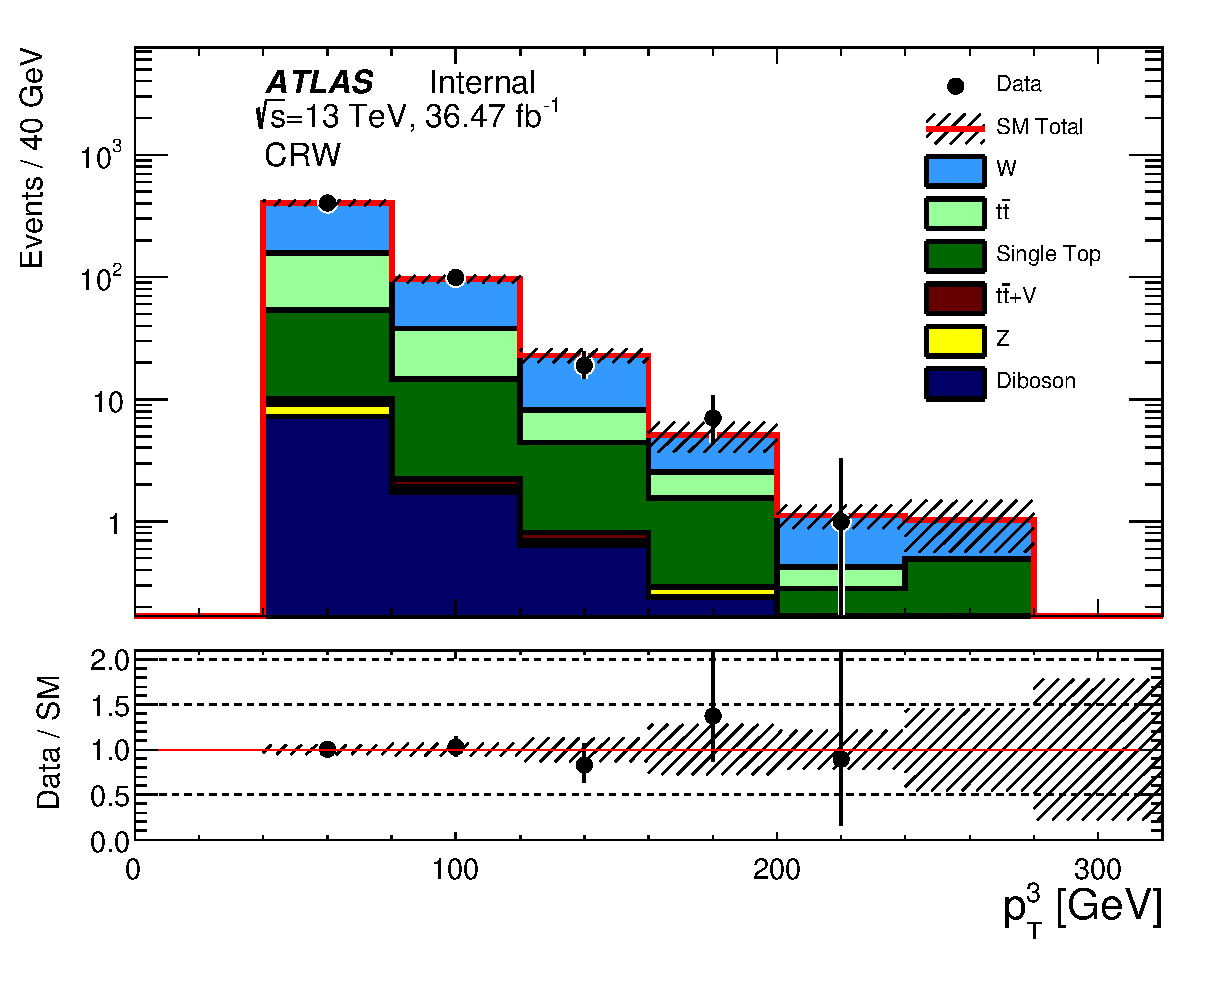
\includegraphics[width=0.45\textwidth]{figures/wJets/postfit/JetPt_3__CRW_log.eps}
  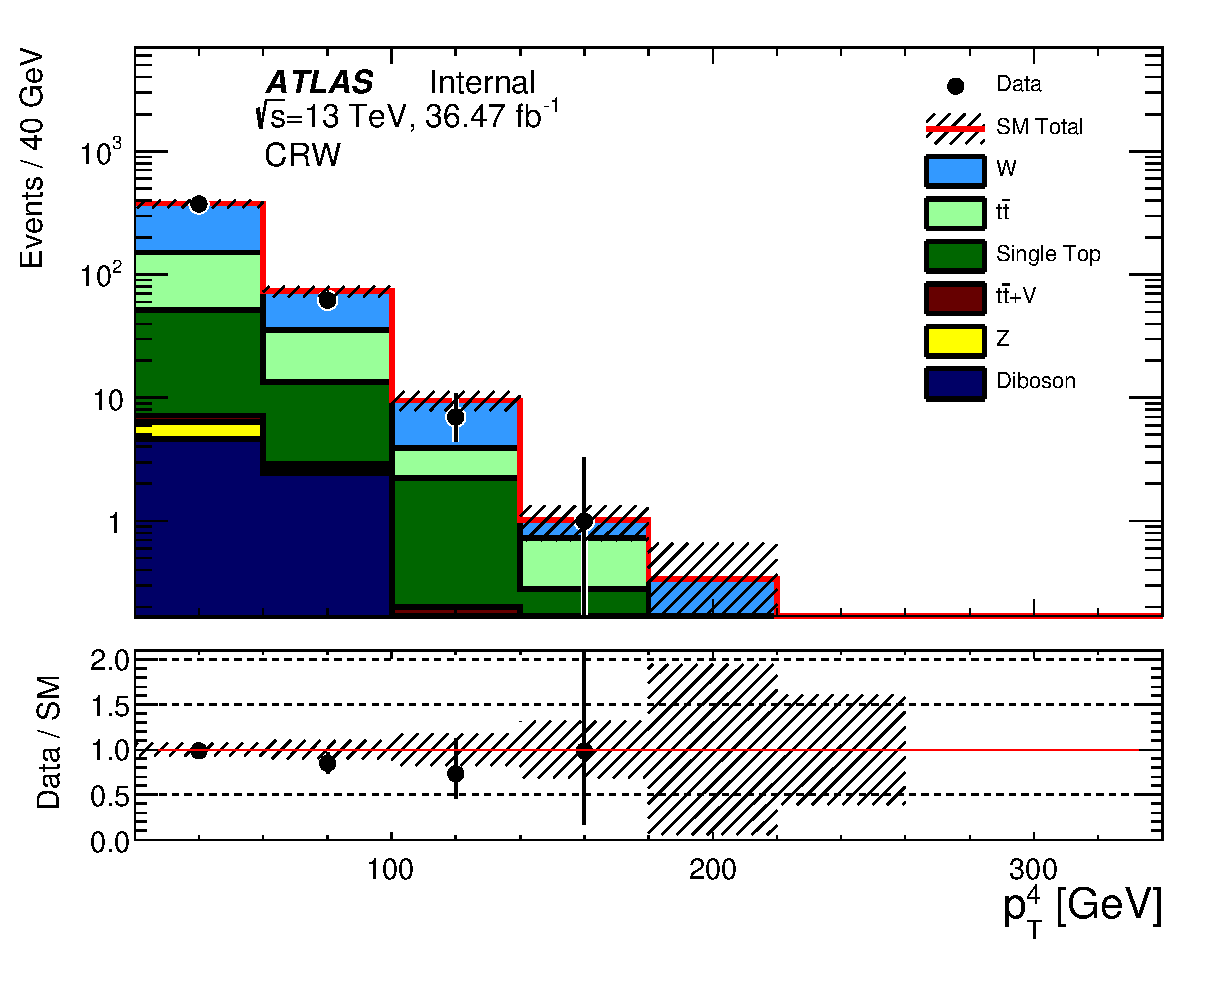
\includegraphics[width=0.45\textwidth]{figures/wJets/postfit/JetPt_4__CRW_log.eps}
  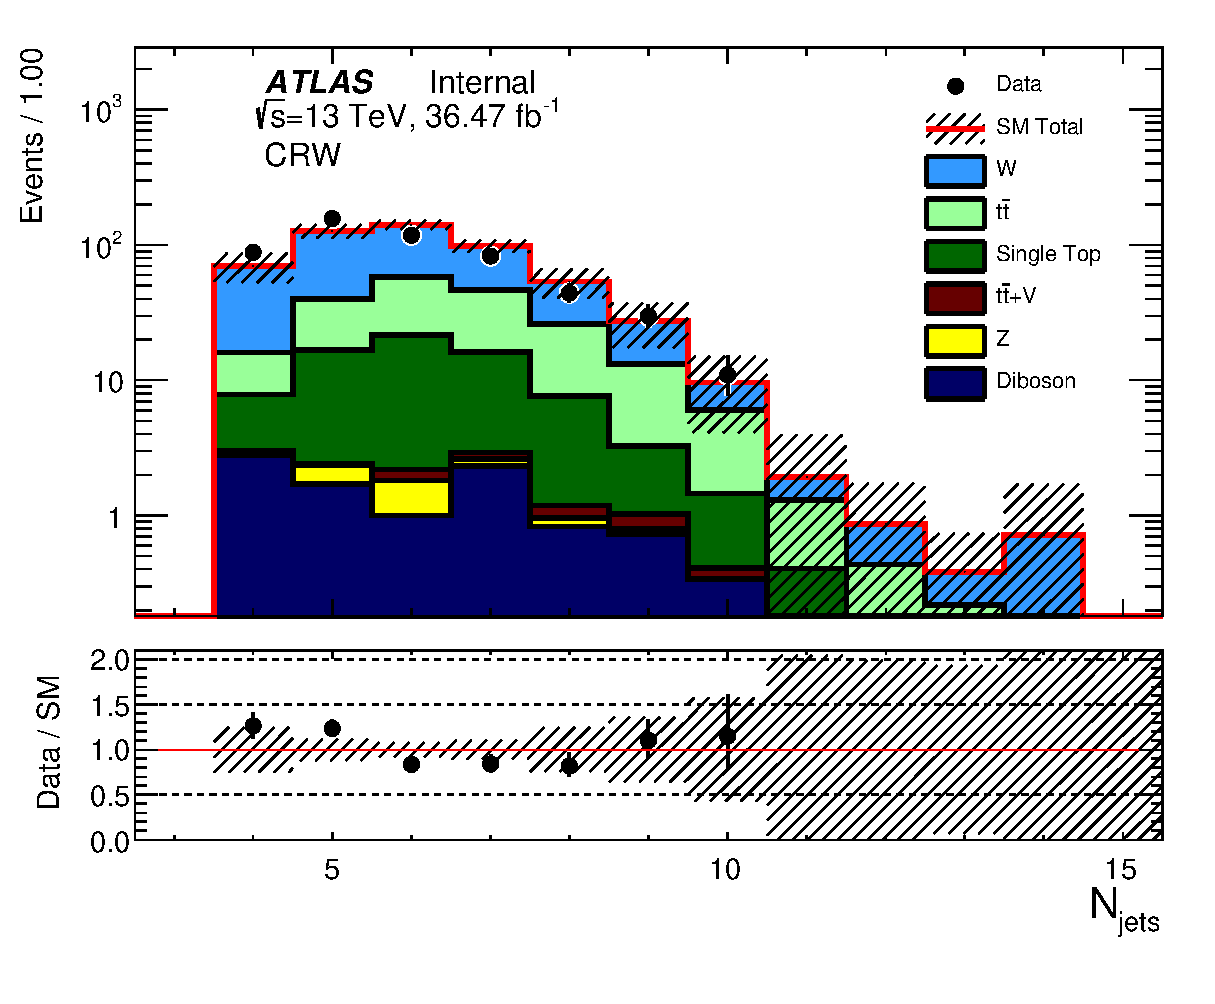
\includegraphics[width=0.45\textwidth]{figures/wJets/postfit/NJets_CRW_log.eps}
  %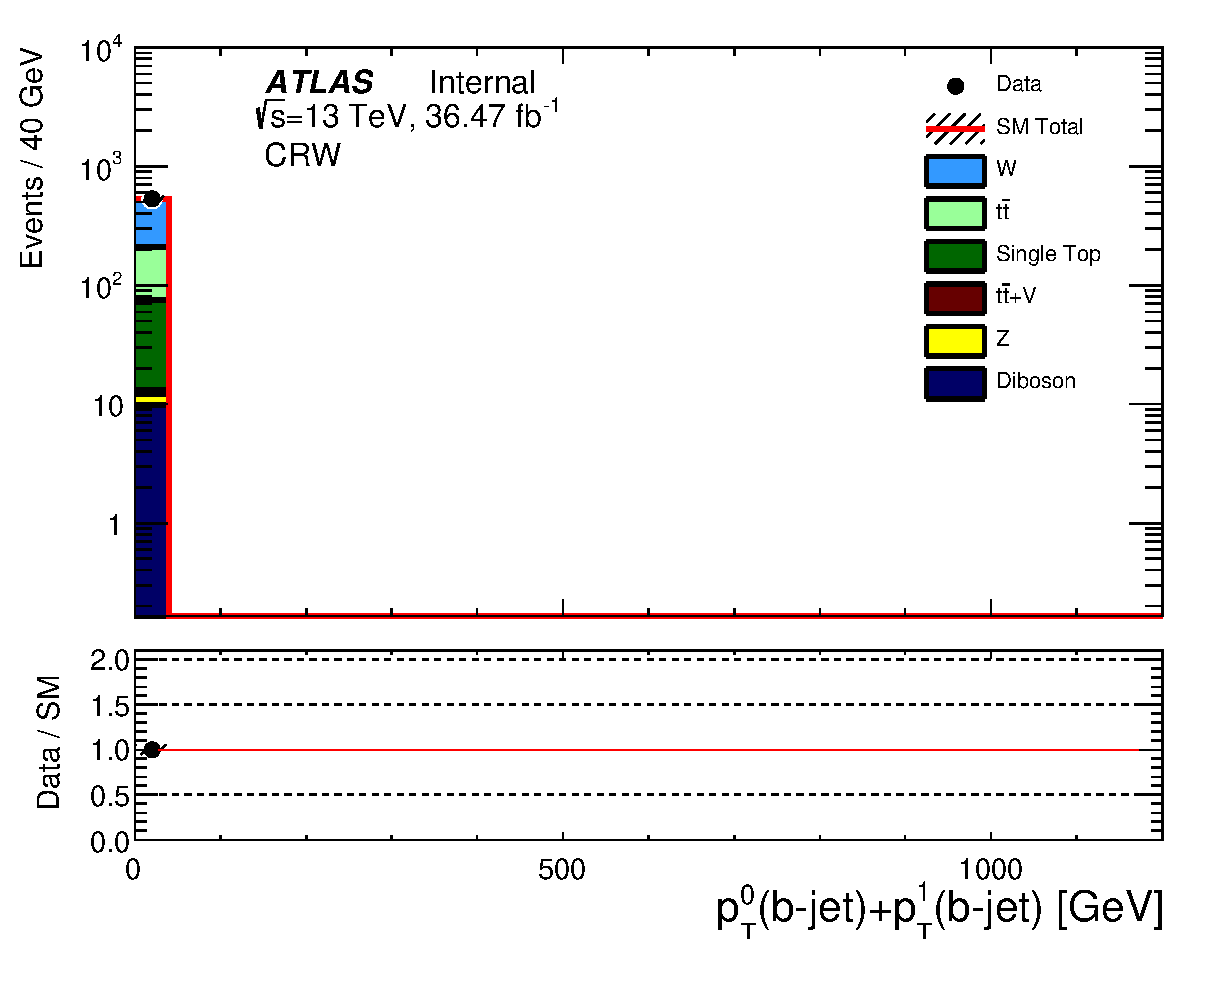
\includegraphics[width=0.45\textwidth]{figures/wJets/postfit/JetPt_JetLeadTagIndex_JetPt_JetSubleadTagIndex__CRW_log.eps}
  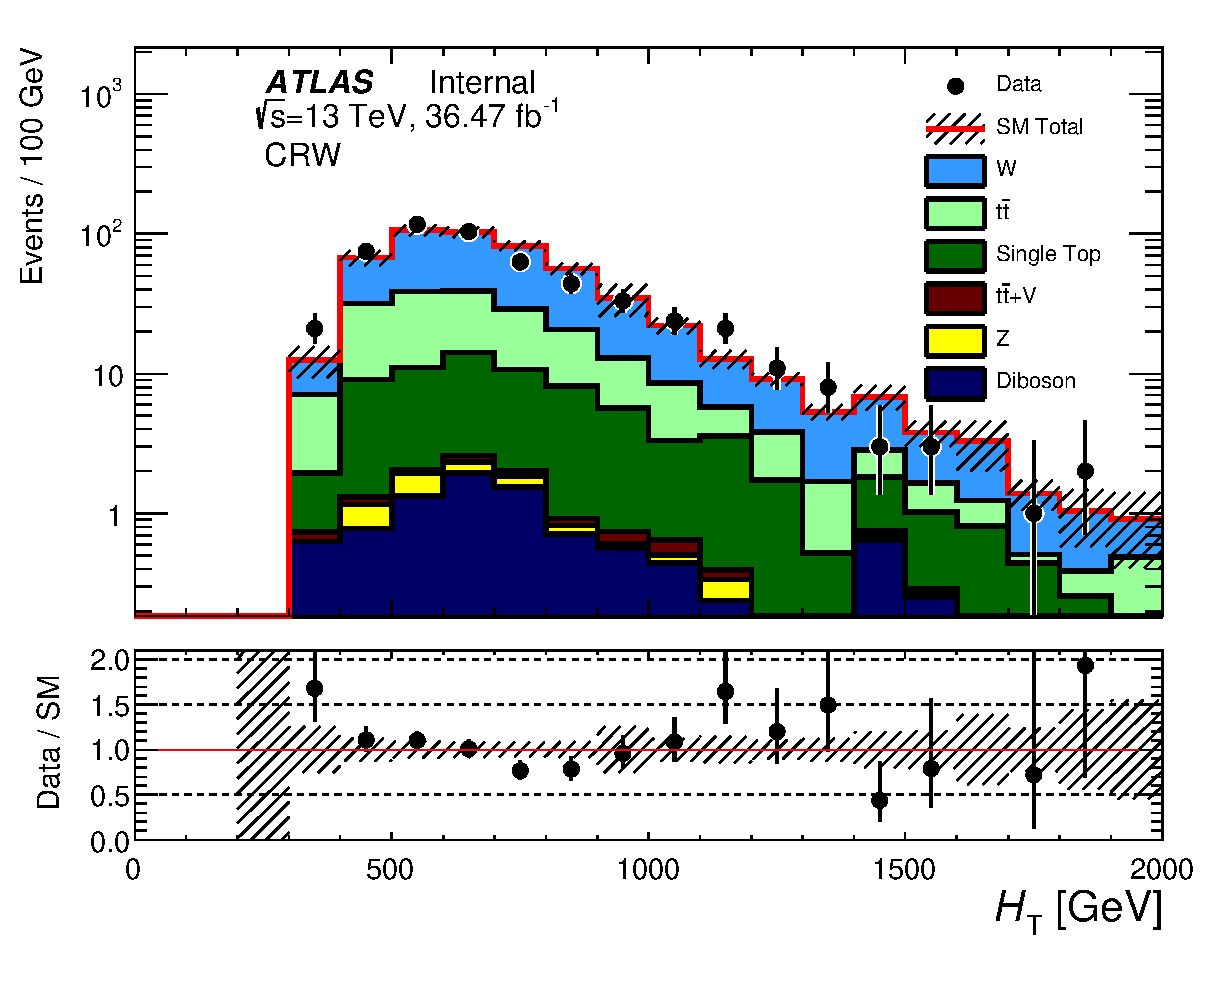
\includegraphics[width=0.45\textwidth]{figures/wJets/postfit/Ht_CRW_log.eps}
  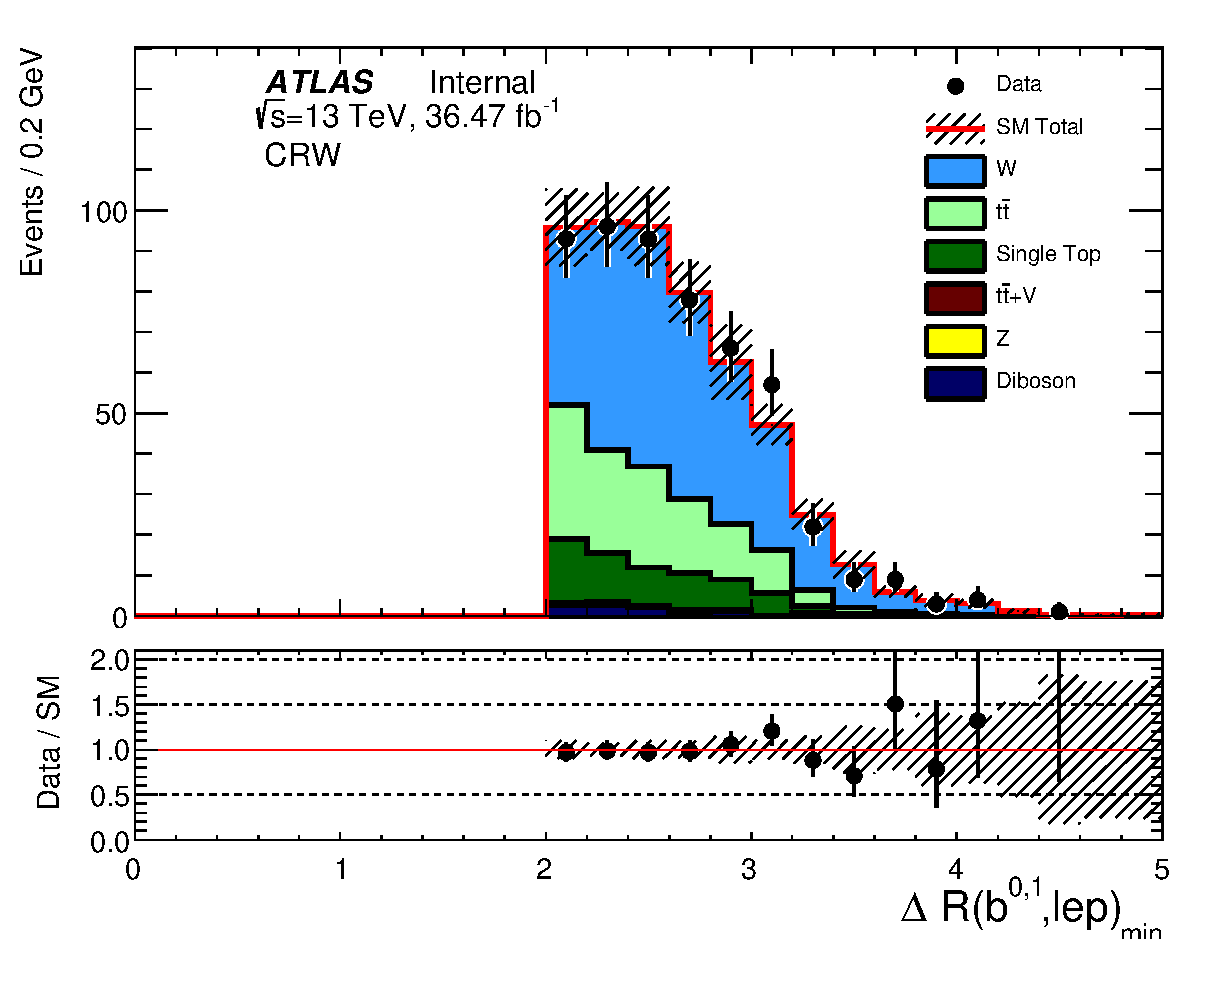
\includegraphics[width=0.45\textwidth]{figures/wJets/postfit/MinDRBLep_CRW.eps}
  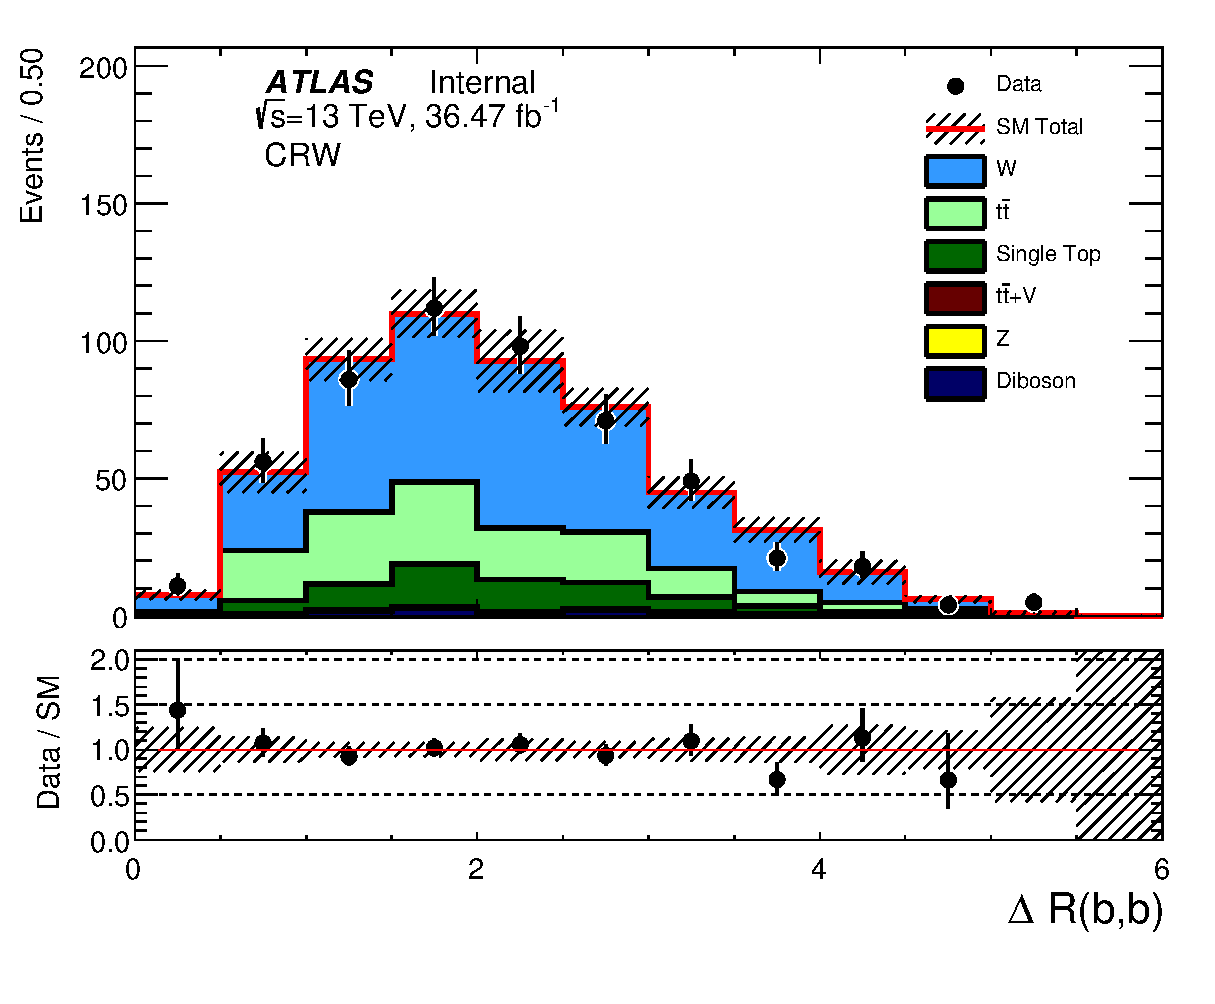
\includegraphics[width=0.45\textwidth]{figures/wJets/postfit/DRBB_CRW.eps}
  \caption{Postfit data/MC comparisons in the CRW. From left to right and top to bottom, the variables shown are the leading four jet \pt, the leading b-tagged jet \pt, \HT, \htsig, \mindrblep, and \drbjetbjet. The background contributions from MC are normalised to \intlumi\ \ifb, and summed together, the data points are shown in black. The hatched band in the ratio shows the MC statistical and detector uncertainties.}
  \label{fig:CRWpts}
\end{figure}

\begin{figure}[!htb]
  \centering
  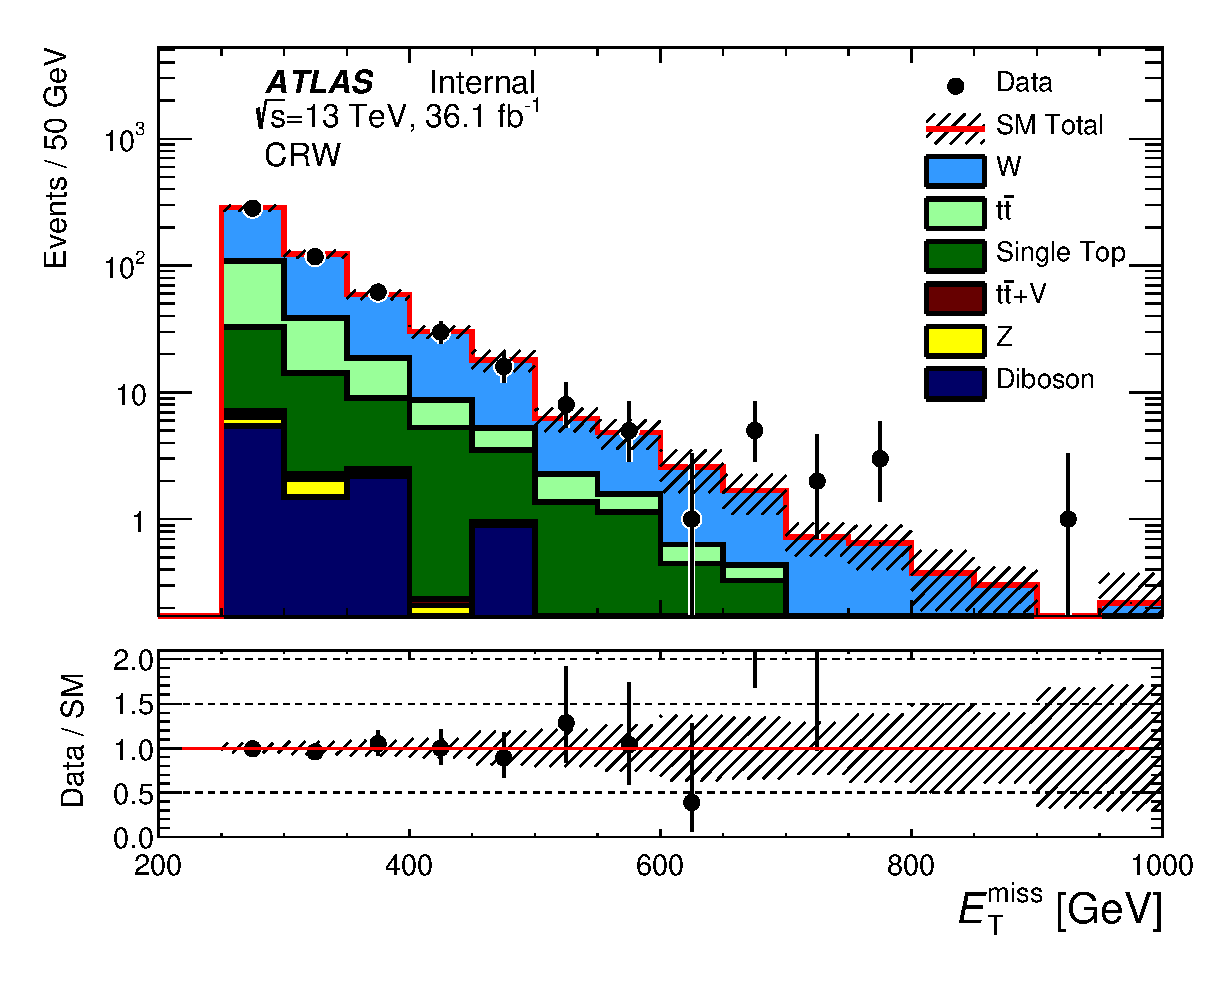
\includegraphics[width=0.45\textwidth]{figures/wJets/postfit/Met_CRW_log.eps}
  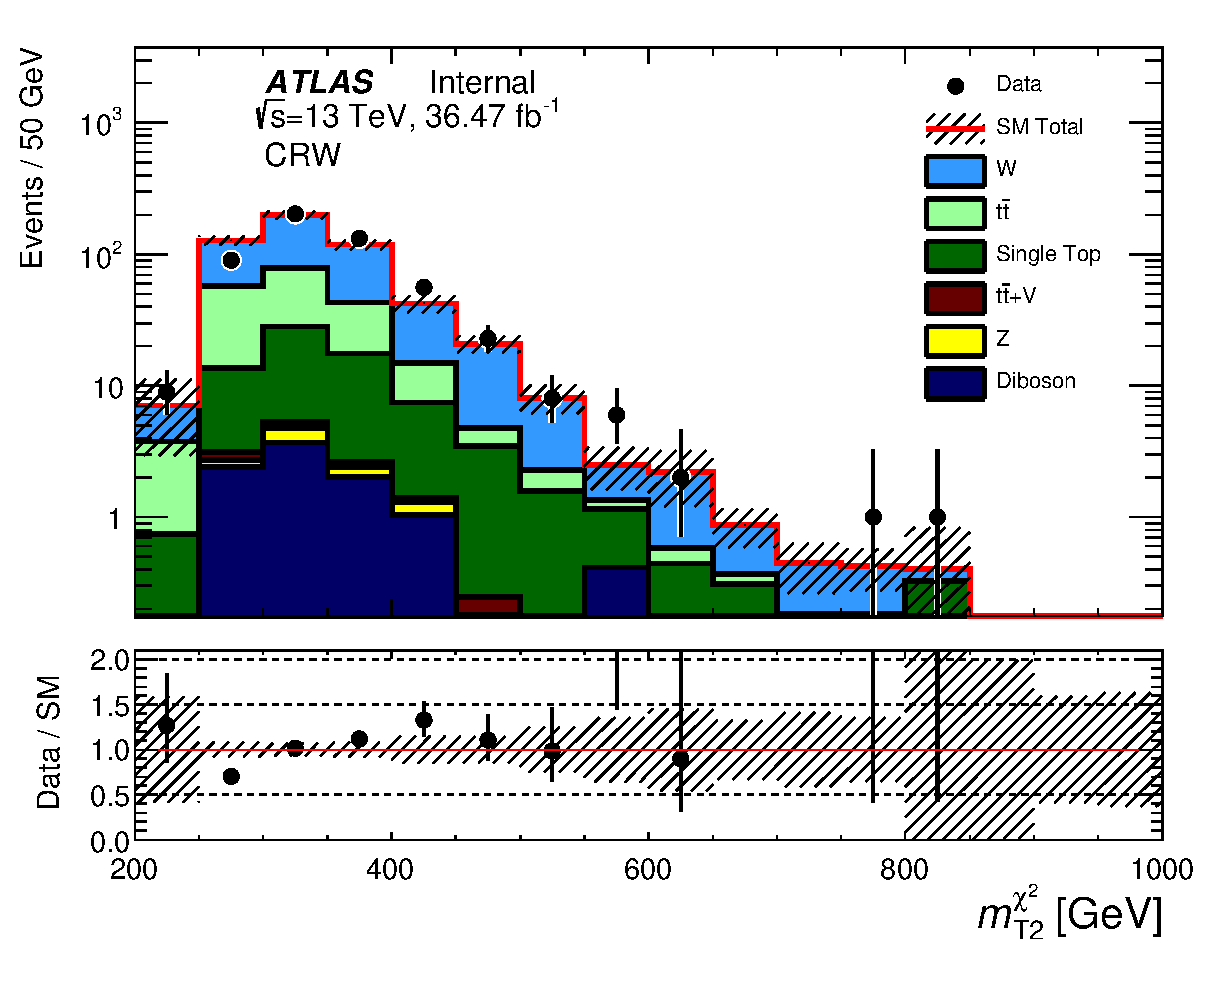
\includegraphics[width=0.45\textwidth]{figures/wJets/postfit/MT2Chi2_CRW_log.eps}
  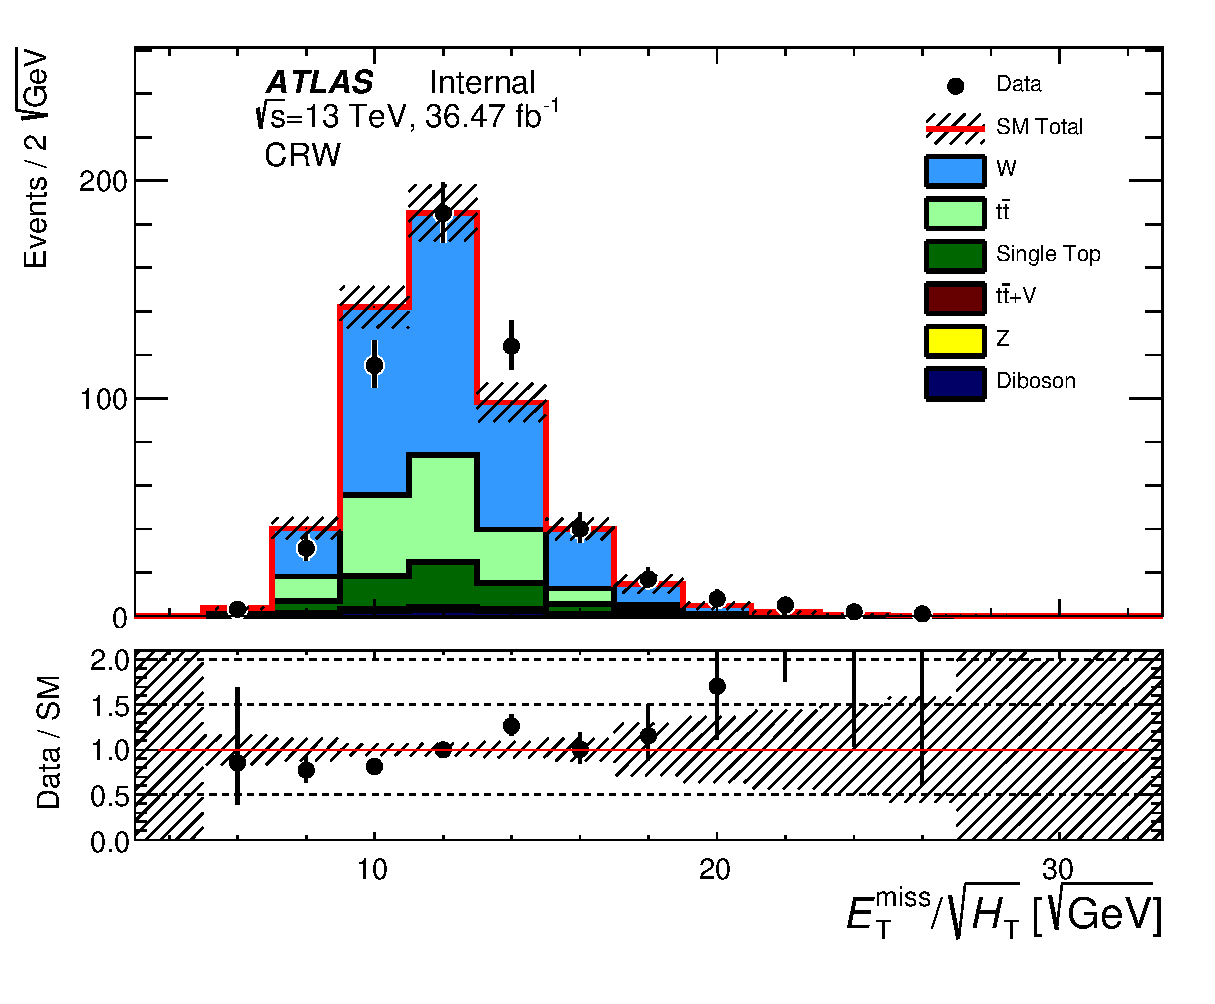
\includegraphics[width=0.45\textwidth]{figures/wJets/postfit/HtSig_CRW.eps}
  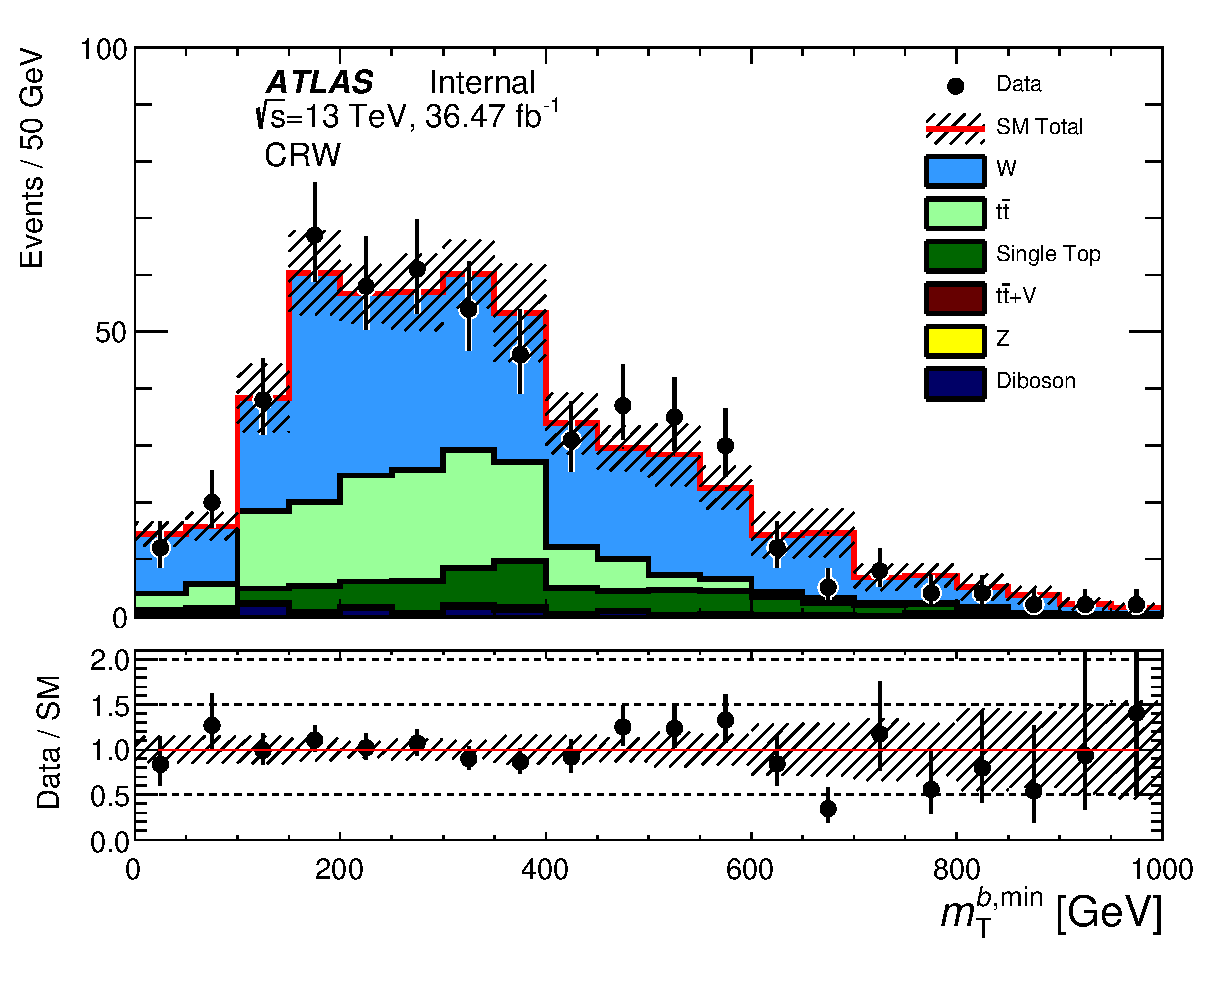
\includegraphics[width=0.45\textwidth]{figures/wJets/postfit/MtBMin_CRW.eps}
  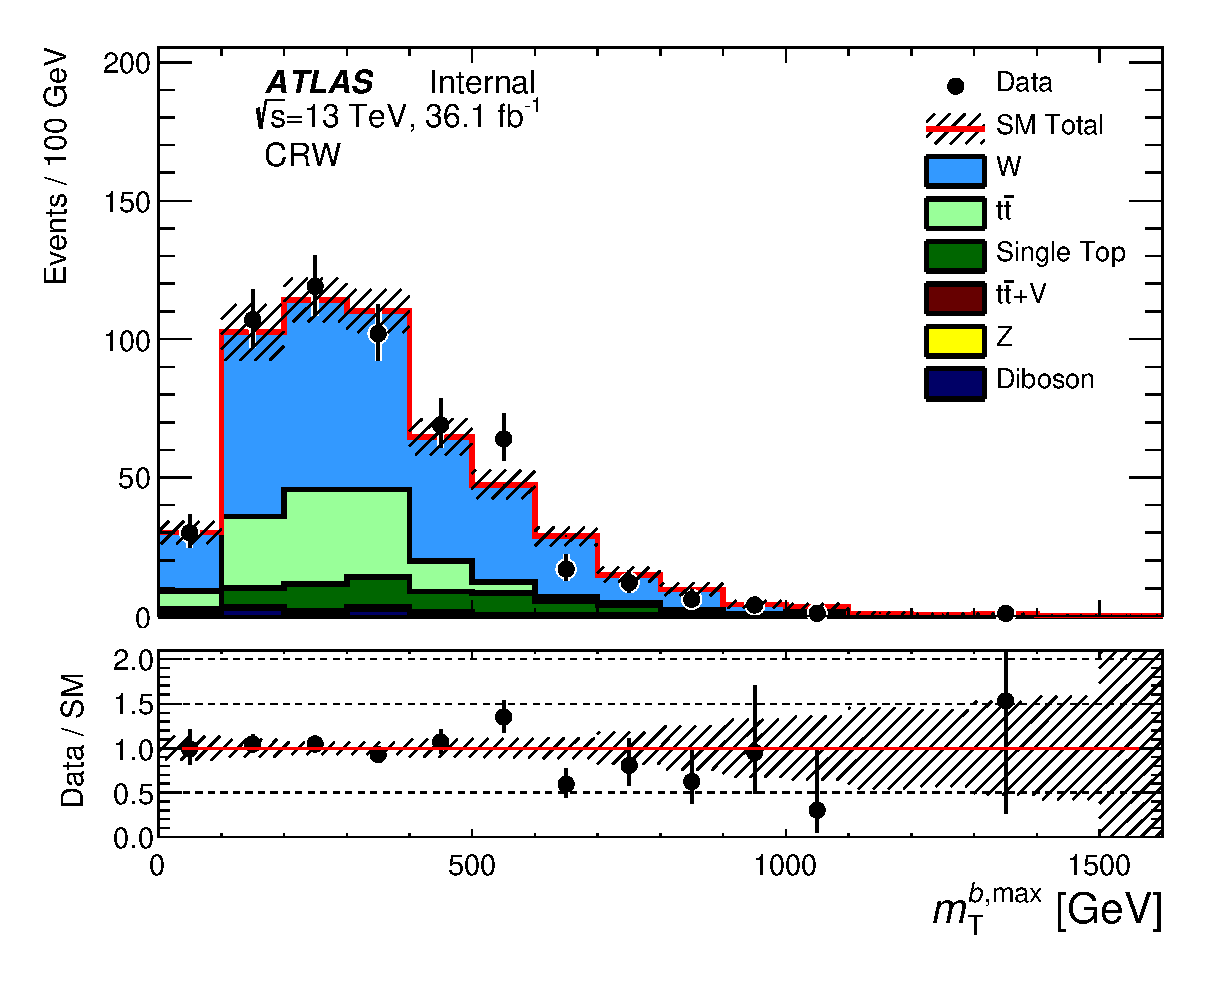
\includegraphics[width=0.45\textwidth]{figures/wJets/postfit/MtBMax_CRW.eps}
  \caption{Postfit data/MC comparisons in the CRW. From left to right and top to bottom, the variables shown are \met, \mtbmin, \mtbmax, \mantikttwelvezero, \mantikttwelveone, and \mantikteightzero. The background contributions from MC are normalised to \intlumi\ \ifb, and summed together, the data points are shown in black. The hatched band in the ratio shows the MC statistical and detecotor uncertainties.}
  \label{fig:CRW}
\end{figure}

\begin{figure}[!htb]
  \centering
  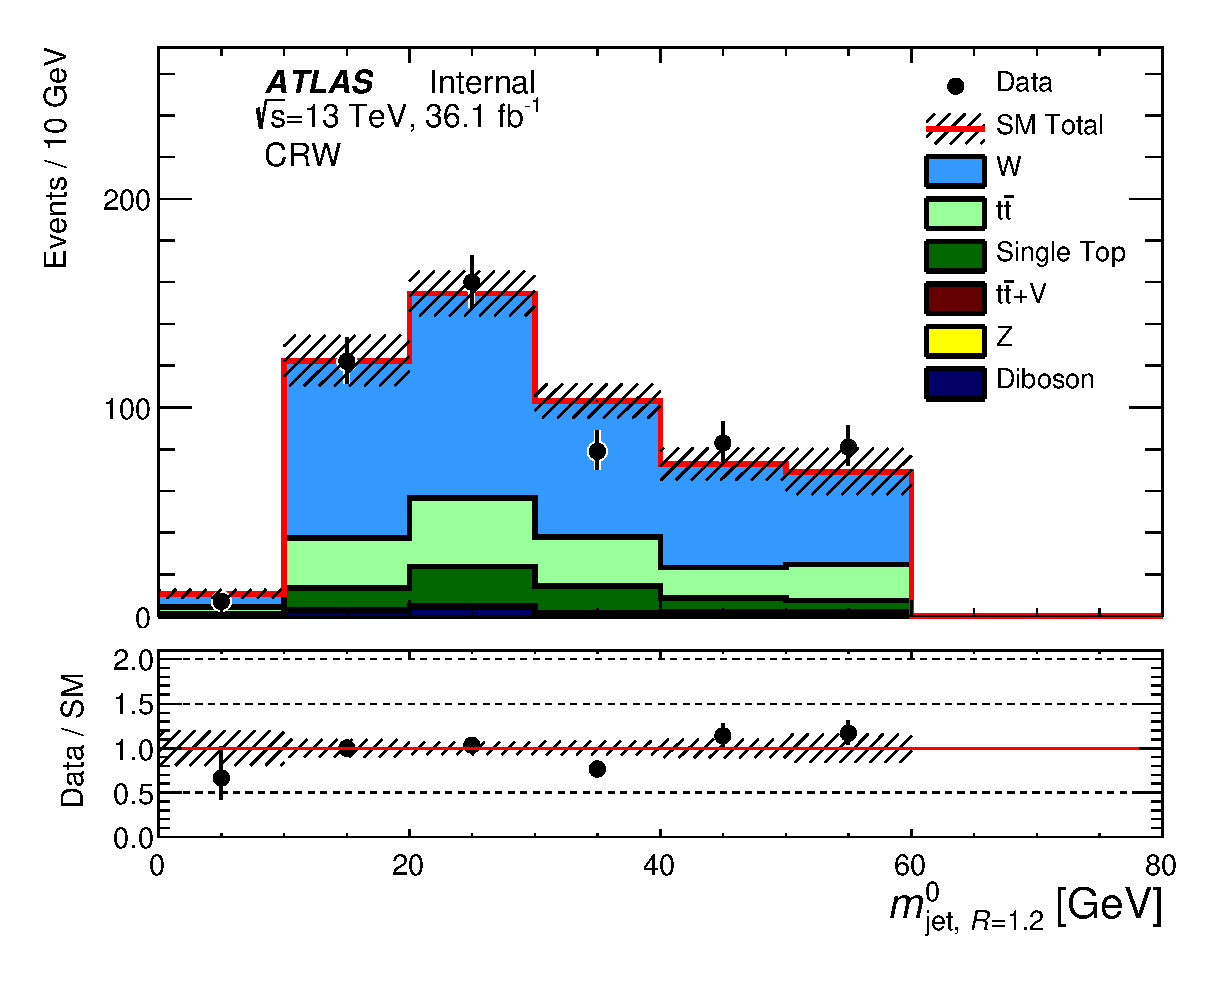
\includegraphics[width=0.45\textwidth]{figures/wJets/postfit/AntiKt12M_0__CRW.eps}
  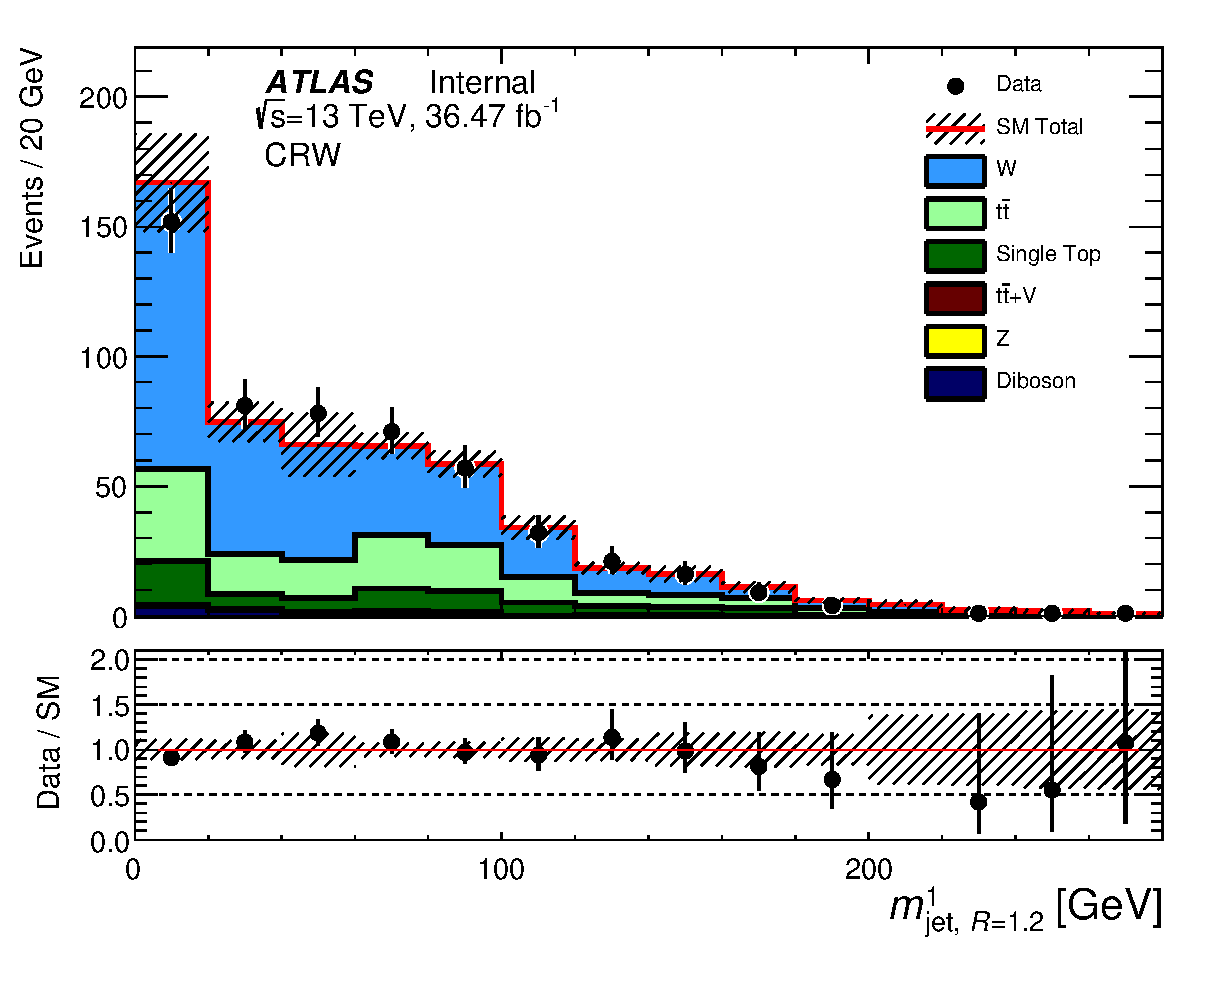
\includegraphics[width=0.45\textwidth]{figures/wJets/postfit/AntiKt12M_1__CRW.eps}
  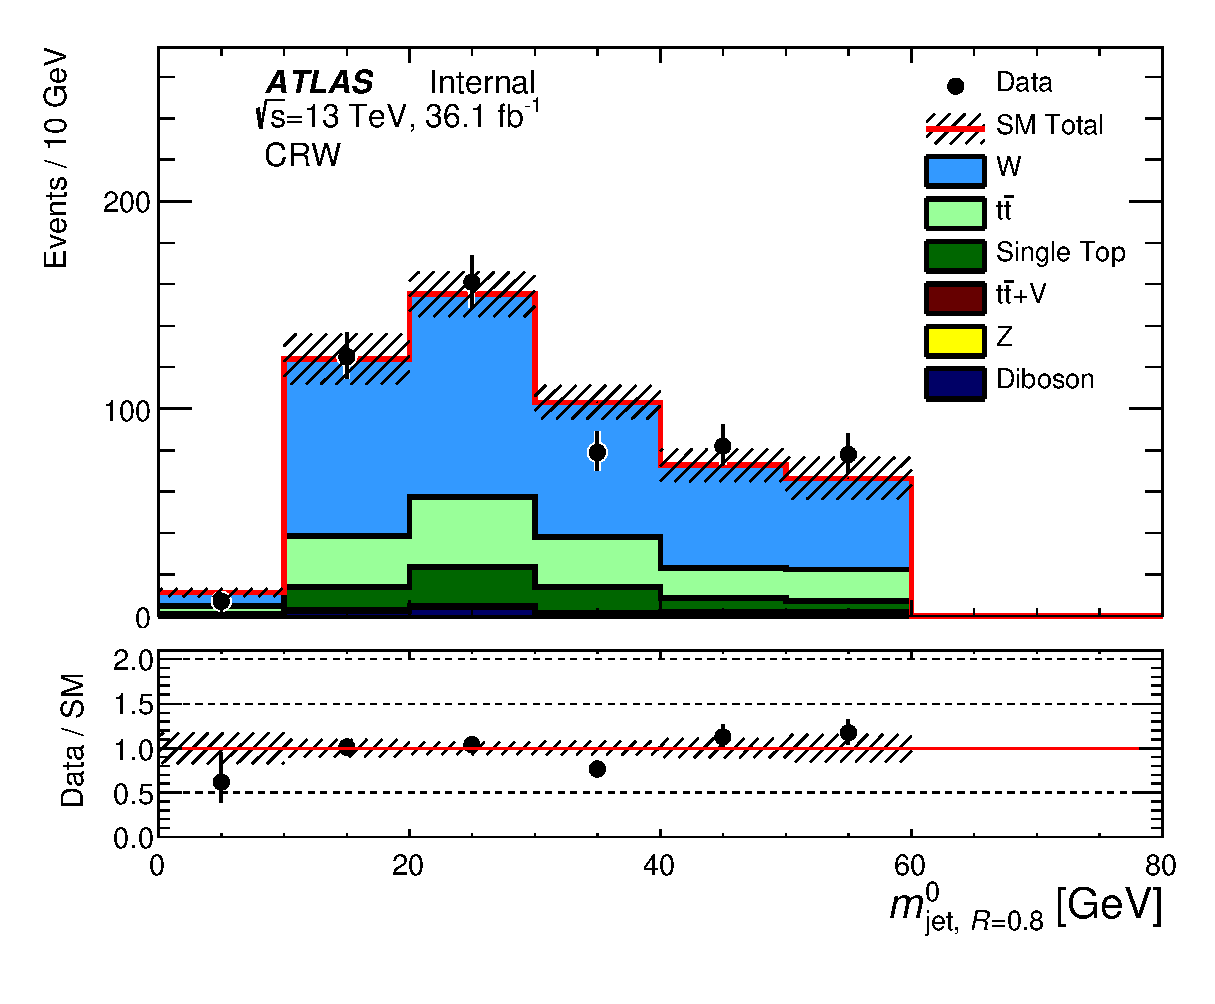
\includegraphics[width=0.45\textwidth]{figures/wJets/postfit/AntiKt8M_0__CRW.eps}
  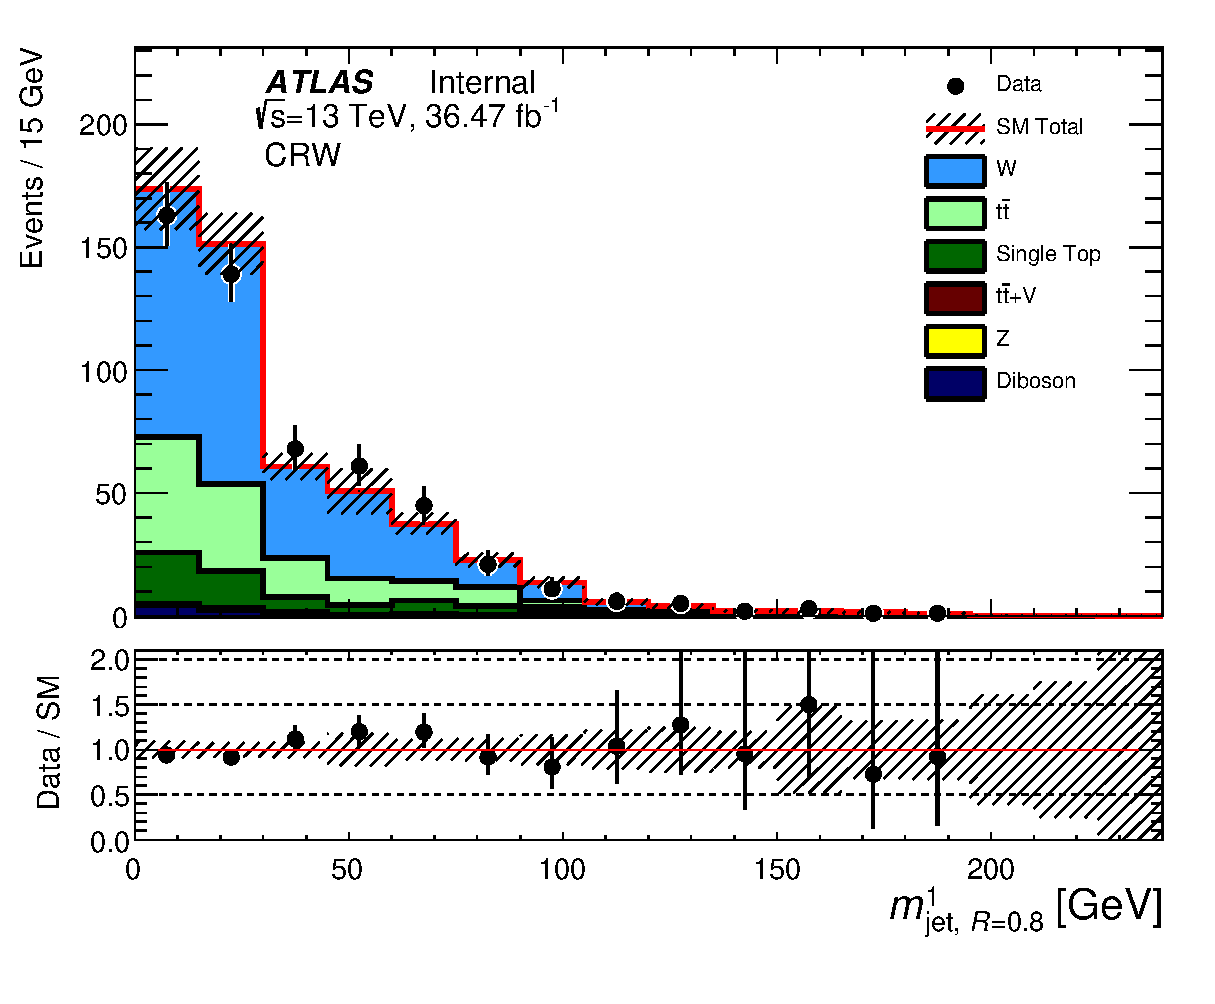
\includegraphics[width=0.45\textwidth]{figures/wJets/postfit/AntiKt8M_1__CRW.eps}
  \caption{Postfit data/MC comparisons in the CRW. From left to right and top to bottom, the variables shown are \met, \mtbmin, \mtbmax, \mantikttwelvezero, \mantikttwelveone, and \mantikteightzero. The background contributions from MC are normalised to \intlumi\ \ifb, and summed together, the data points are shown in black. The hatched band in the ratio shows the MC statistical and detecotor uncertainties.}
  \label{fig:CRWMasses}
\end{figure}

\clearpage

\subsubsection{\Wjets\ Validation Region}
\label{section:VRW}

The selections for a possible \Wjets\ validation region in the 1-lepton, two b-jets channel (VRW) are summarised in Tab.~\ref{tab:VRW}.

\begin{table}[htpb]
  \caption{Summary of the selection for the 1-lepton $W$+jets validation region. The signal lepton is treated as a jet. The same \met\ triggers as mentioned in Table~\ref{tab:SRcommon} are used.}
  \begin{center}
    \begin{tabular}{c|c}
      \hline \hline
                                          & VRW              \\ \hline
      Number of leptons                   & 1                \\ \hline
      Number of jets (incl. lepton)       & $\geq 4$         \\ \hline
      $\pt$ of jets (incl. lepton) in GeV & (80,80,40,40)    \\ \hline
      Number of $b$-jets                  & $\geq 2$         \\ \hline
      \mindphijettwomet                   & $>0.4$           \\ \hline
      $\met$                              & $>250$ GeV       \\ \hline
      \mtlepmet                           & $>30$,$<100$ GeV \\ \hline
      \mantikttwelvezero                  & $<70\,$GeV       \\ \hline
      \mtbmin                             & 150 GeV          \\ \hline
      \mindrblep                          & $>1.8$           \\ \hline \hline
    \end{tabular}
  \end{center}
  \label{tab:VRW}
\end{table}

The yields in the VRW region are summarised in Tab.~\ref{tab:VRW_yields}. The \Wjets\ purity in this region is 30\% while the signal contamination is less than 15\% for all signal benchmark points except for ($\mstop$, $m_{\chinoonepm}$, $\mLSP$) = (550, 100, 50) GeV which has been excluded in previous searches. 

\begin{table}[!htb]
  \centering
  \begin{tabular}{c|c}
\hline\hline
\multicolumn{2}{c}{\bf VRW (38\% purity)} \\ \hline 
Z & 0.21 $\pm$ 0.07 \\
dibosons & 3.05 $\pm$ 0.89 \\
ttbar & 35.72 $\pm$ 2.02 \\
singleTop & 42.62 $\pm$ 1.47 \\
ttV & 0.57 $\pm$ 0.13 \\
W & 50.45 $\pm$ 3.50 \\
\hline
Total MC & 132.63 $\pm$ 4.40 \\
Data & 140.00 $\pm$ 11.83 \\
 \hline
SF & 1.15 $\pm$ 0.31 \\
\hline\hline
\end{tabular}

  \caption{Yields in the VRW in \intlumi\ \ifb\ of data. The uncertainty on the SF, which is compatible within statistical uncertainties with the SF from the CR, should come down significantly. }
  \label{tab:VRW_yields}
\end{table}

A selection of distributions where data is compared to MC (no normalisation factors applied) is shown in Fig.~\ref{fig:VRW}. 

\begin{figure}[!htb]
  \centering
  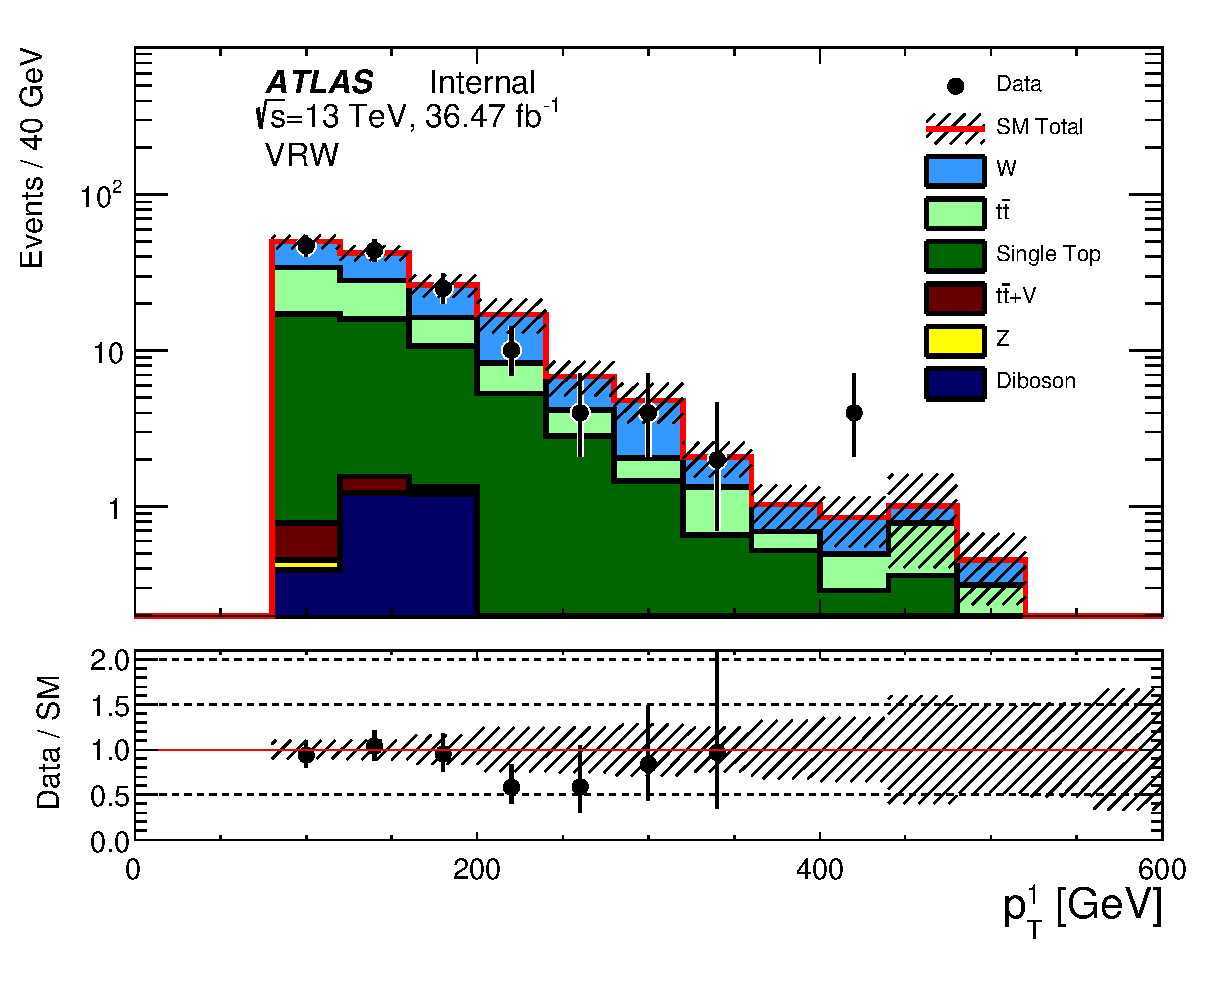
\includegraphics[width=0.45\textwidth]{figures/wJets/postfit/JetPt_1__VRW_log.eps}
  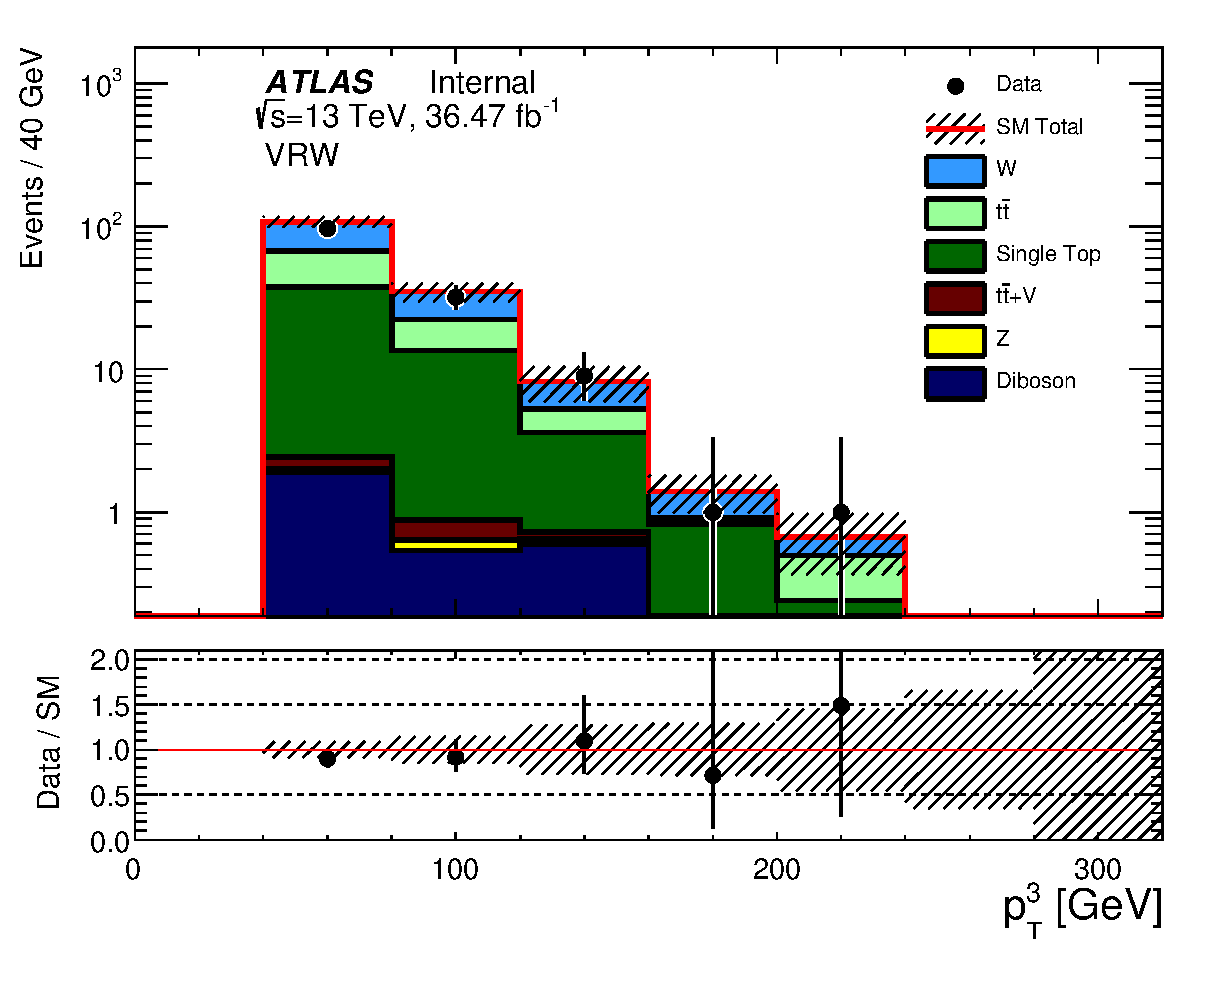
\includegraphics[width=0.45\textwidth]{figures/wJets/postfit/JetPt_3__VRW_log.eps}
  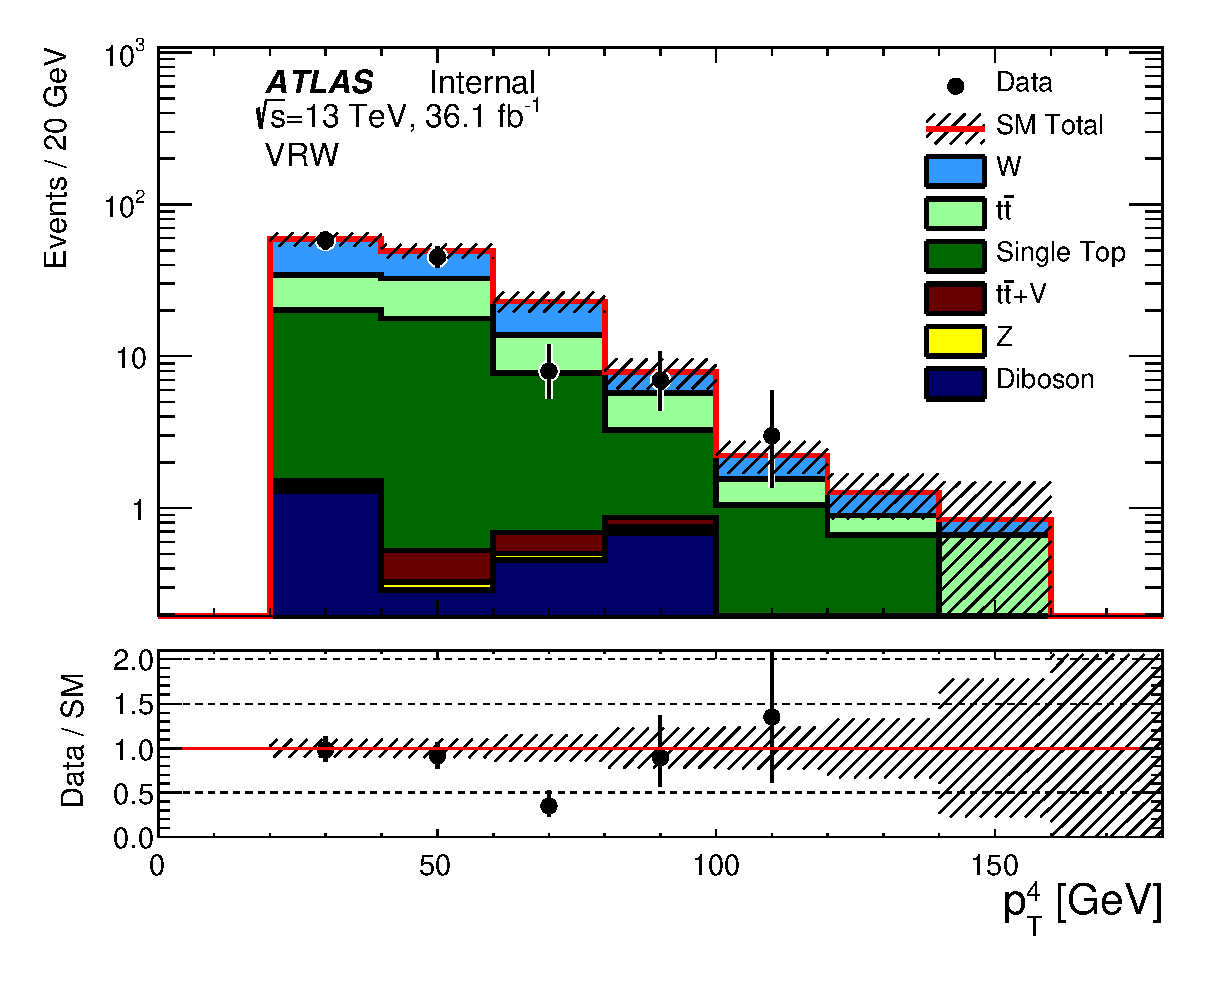
\includegraphics[width=0.45\textwidth]{figures/wJets/postfit/JetPt_4__VRW_log.eps}
  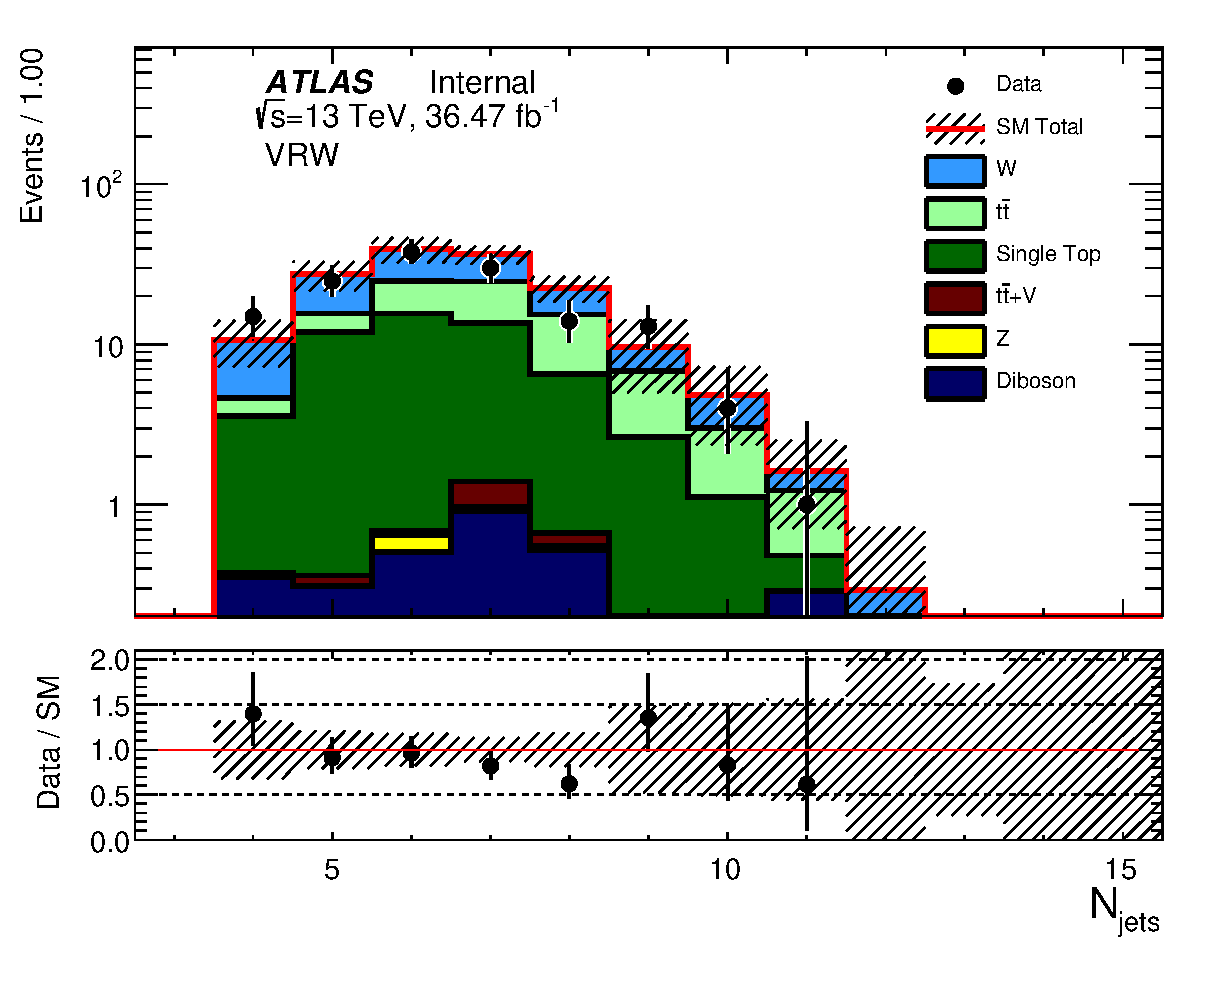
\includegraphics[width=0.45\textwidth]{figures/wJets/postfit/NJets_VRW_log.eps}
  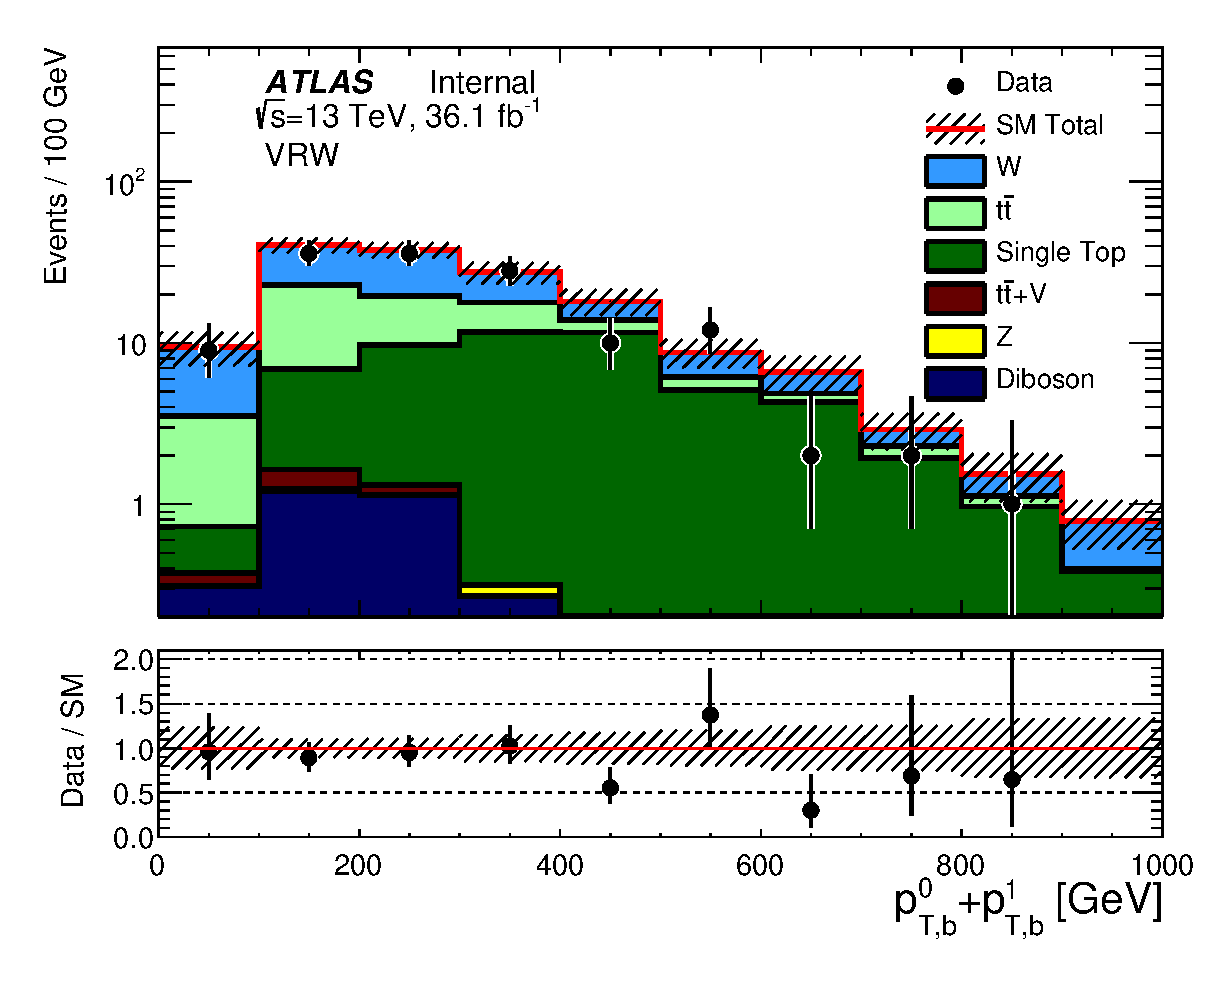
\includegraphics[width=0.45\textwidth]{figures/wJets/postfit/JetPt_JetLeadTagIndex_JetPt_JetSubleadTagIndex__VRW_log.eps}
  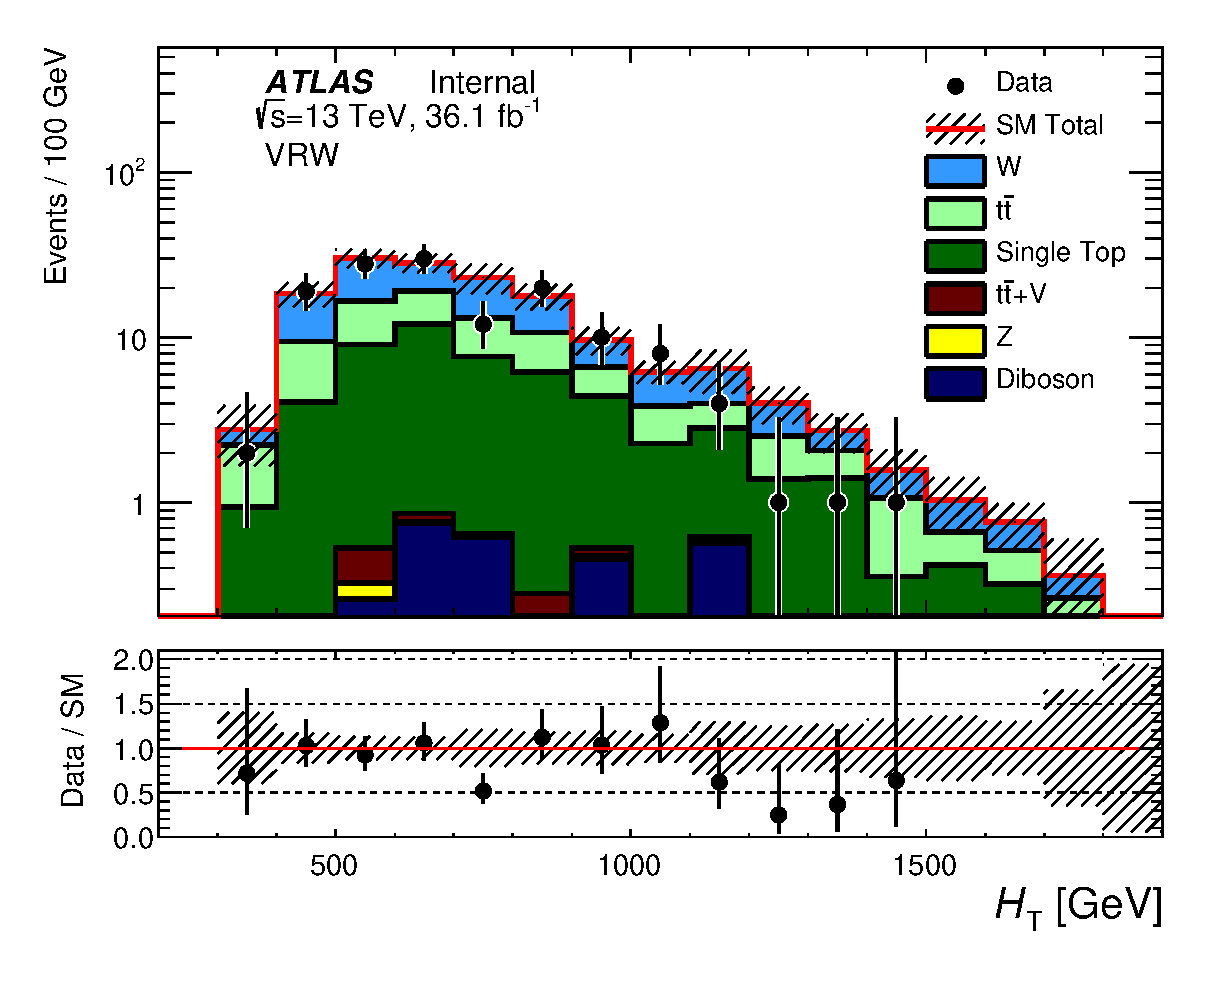
\includegraphics[width=0.45\textwidth]{figures/wJets/postfit/Ht_VRW_log.eps}
  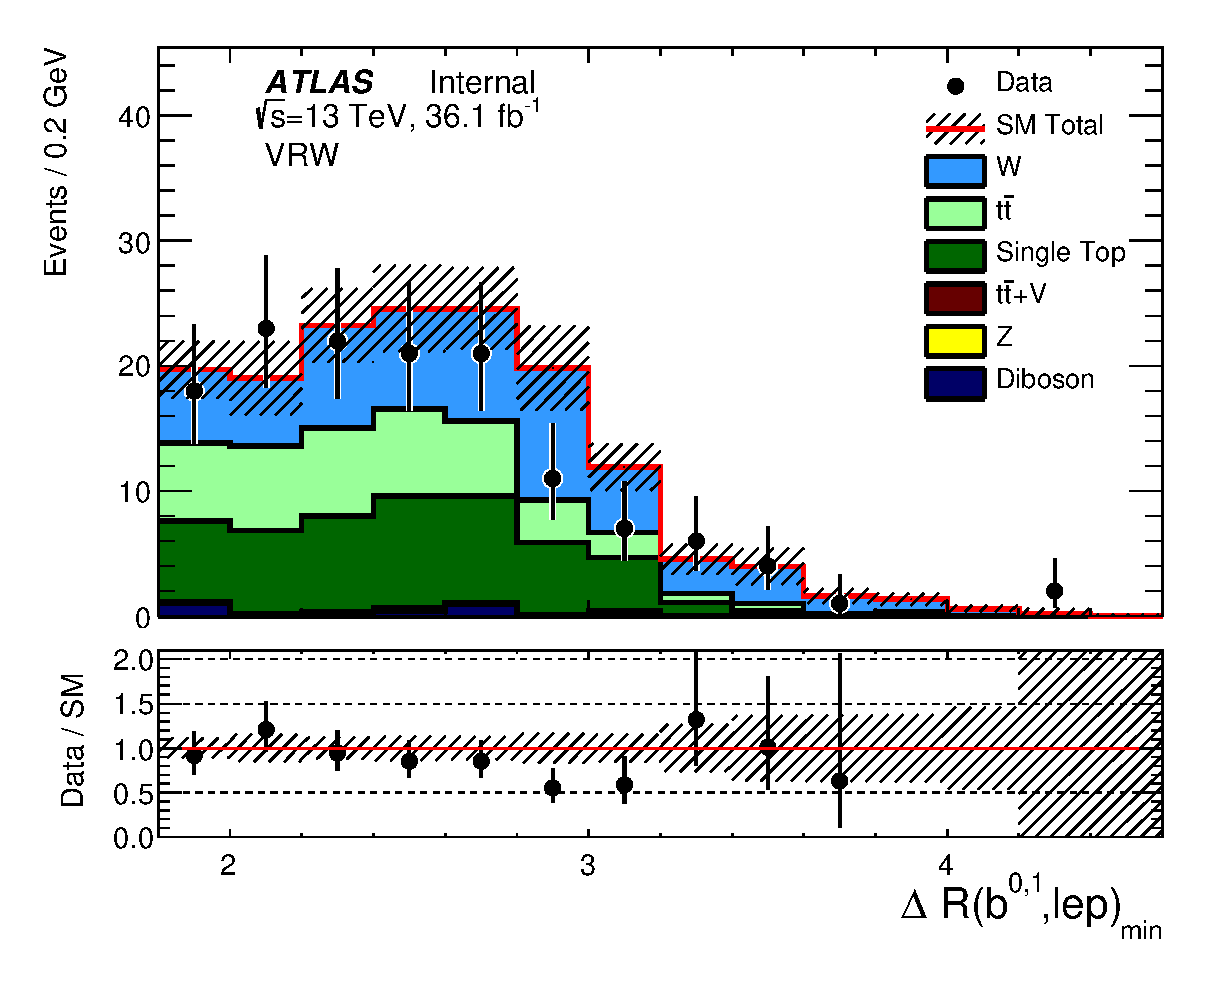
\includegraphics[width=0.45\textwidth]{figures/wJets/postfit/MinDRBLep_VRW.eps}
  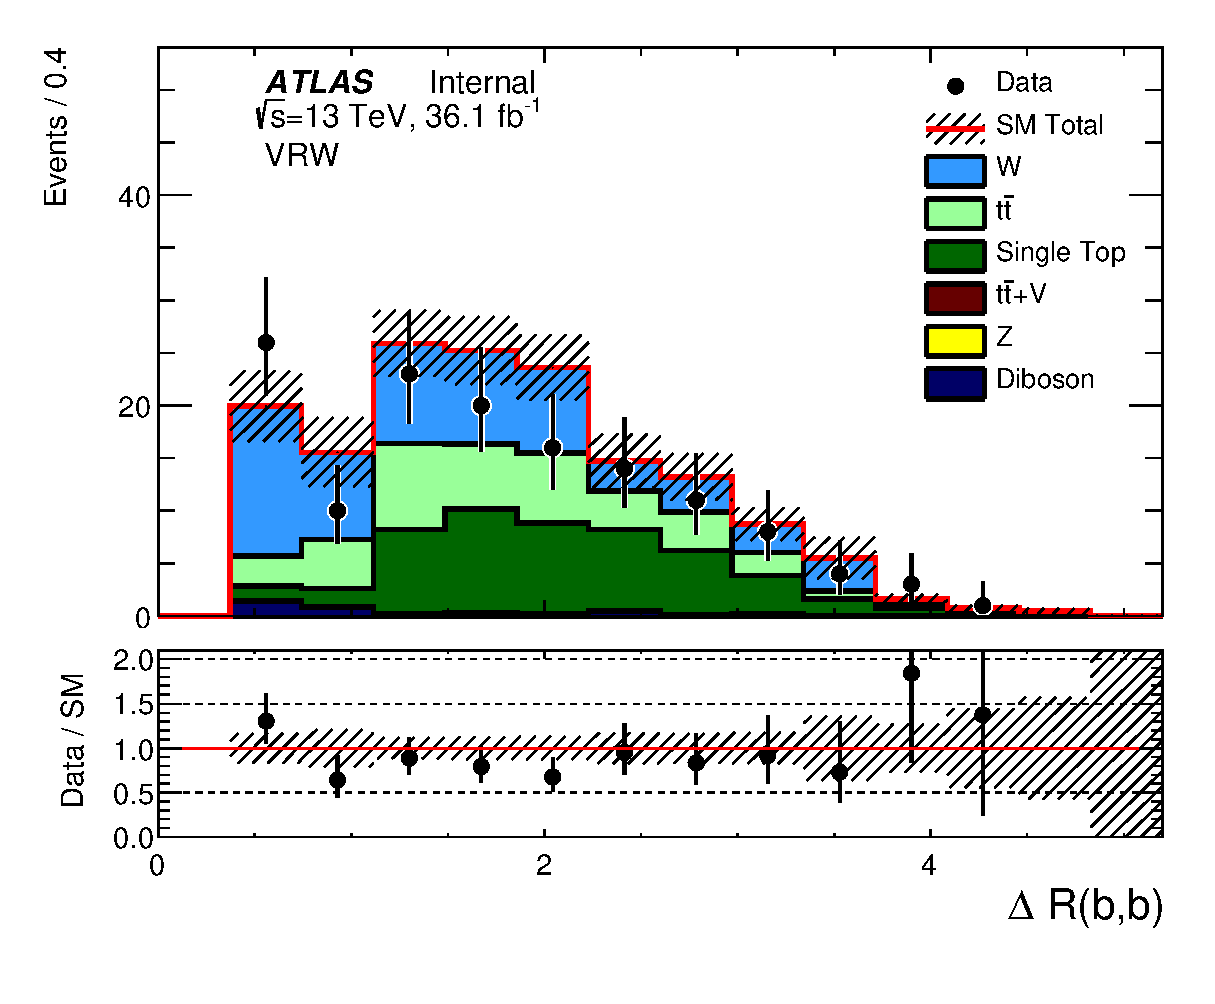
\includegraphics[width=0.45\textwidth]{figures/wJets/postfit/DRBB_VRW.eps}
  \caption{Postfit data/MC comparisons in the VRW. From left to right and top to bottom, the variables shown are the leading four jet \pt, the leading b-tagged jet \pt, \HT, \htsig, \mindrblep, and \drbjetbjet. The background contributions from MC are normalised to \intlumi\ \ifb, and summed together, the data points are shown in black. The hatched band in the ratio shows the MC statistical and detector uncertainties.}
  \label{fig:VRWpts}
\end{figure}

\begin{figure}[!htb]
  \centering
  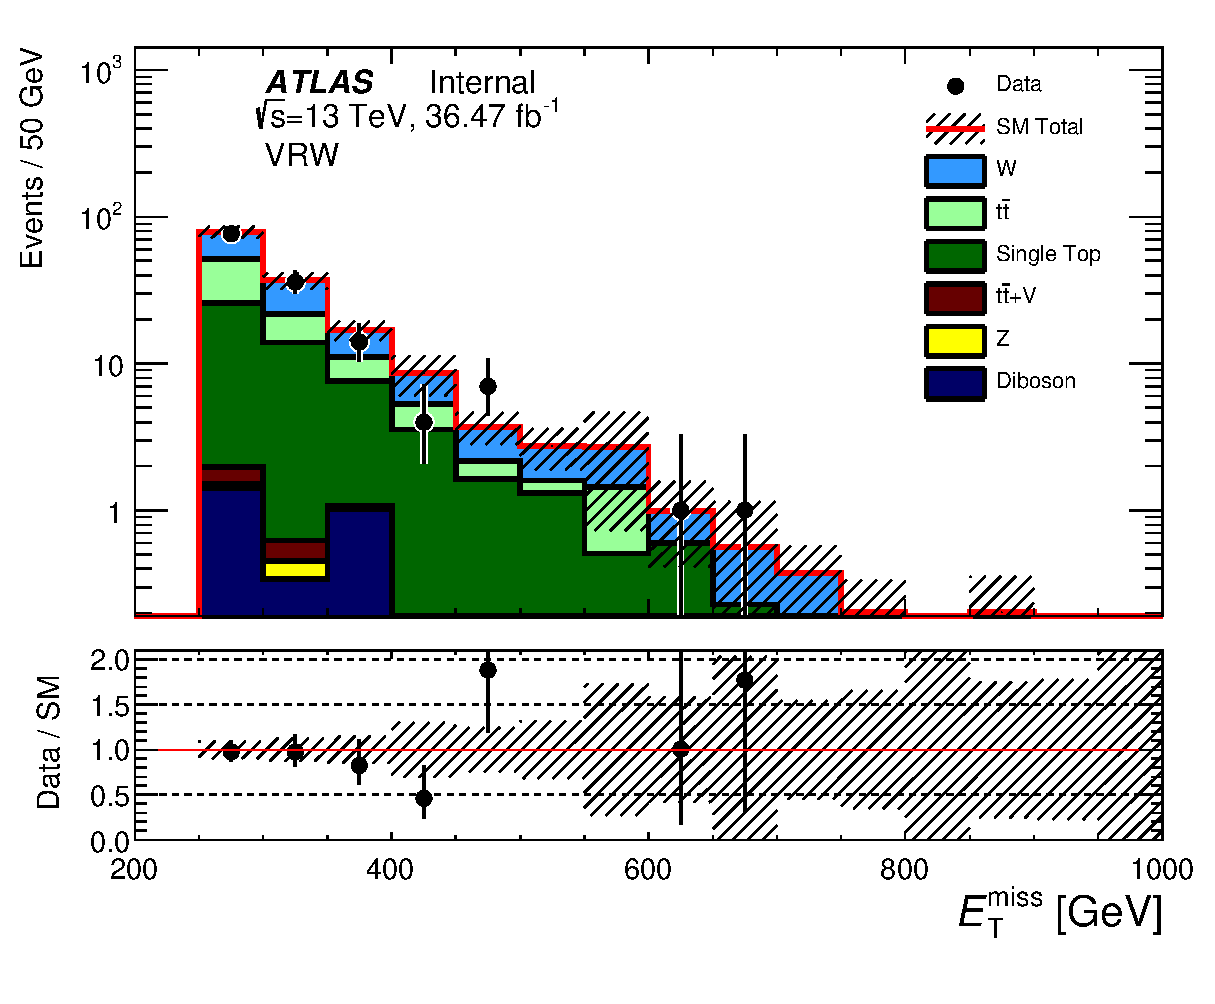
\includegraphics[width=0.45\textwidth]{figures/wJets/postfit/Met_VRW_log.eps}
  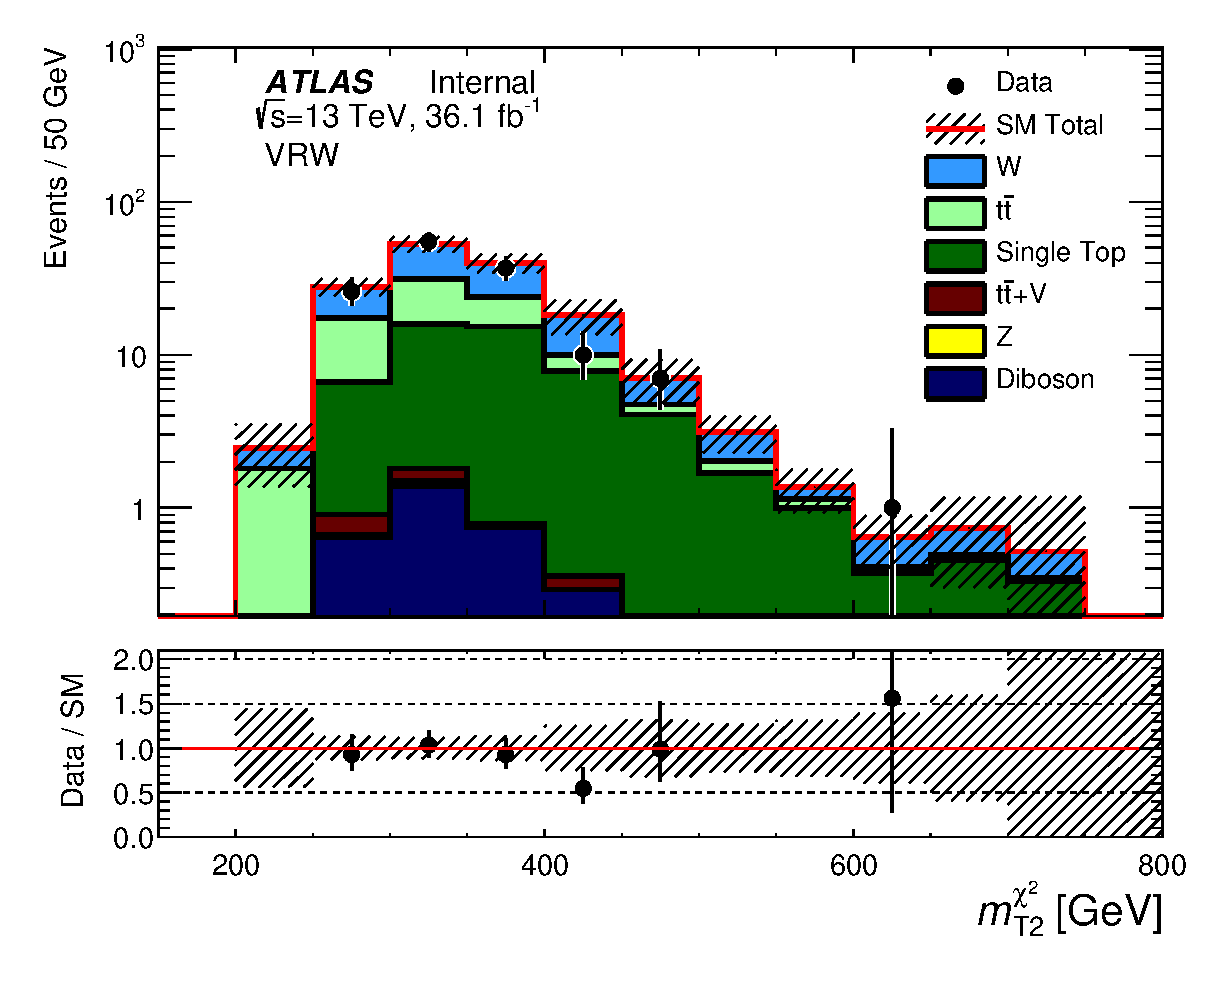
\includegraphics[width=0.45\textwidth]{figures/wJets/postfit/MT2Chi2_VRW_log.eps}
  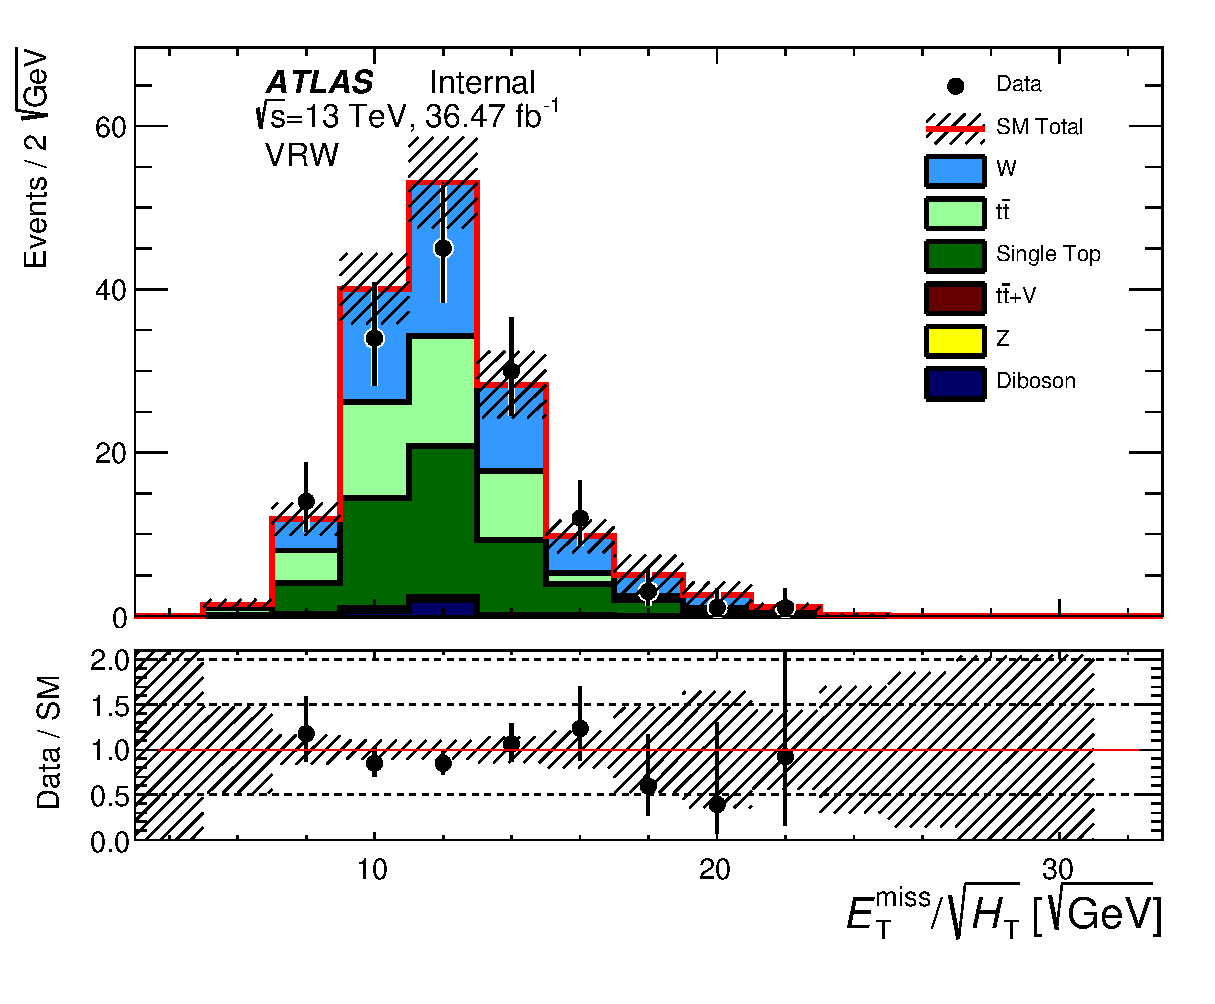
\includegraphics[width=0.45\textwidth]{figures/wJets/postfit/HtSig_VRW.eps}
  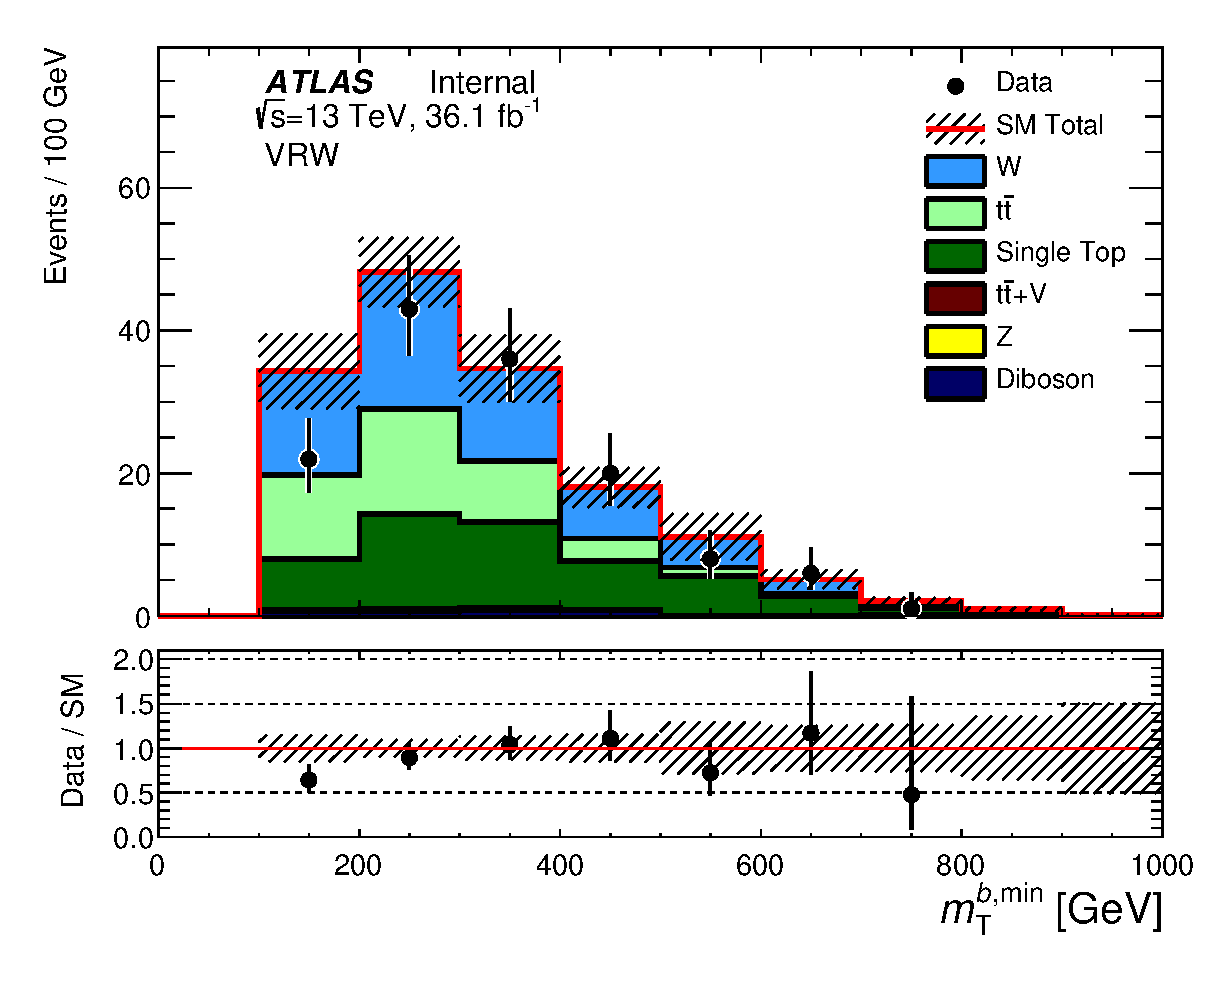
\includegraphics[width=0.45\textwidth]{figures/wJets/postfit/MtBMin_VRW.eps}
  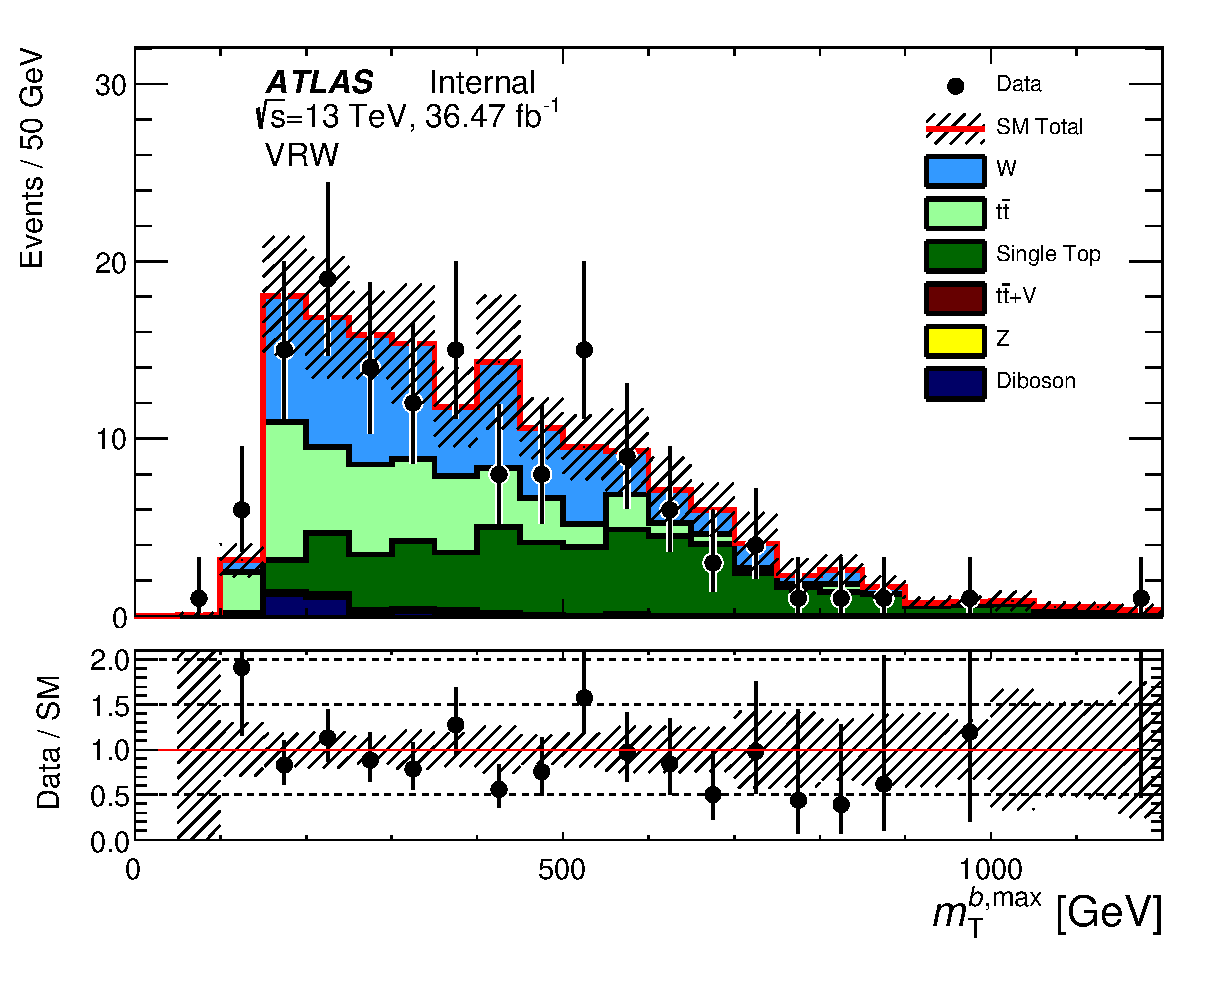
\includegraphics[width=0.45\textwidth]{figures/wJets/postfit/MtBMax_VRW.eps}
  \caption{Postfit data/MC comparisons in the VRW. From left to right and top to bottom, the variables shown are \met, \mtbmin, \mtbmax, \mantikttwelvezero, \mantikttwelveone, and \mantikteightzero. The background contributions from MC are normalised to \intlumi\ \ifb, and summed together, the data points are shown in black. The hatched band in the ratio shows the MC statistical and detecotor uncertainties.}
  \label{fig:VRW}
\end{figure}

\begin{figure}[!htb]
  \centering
  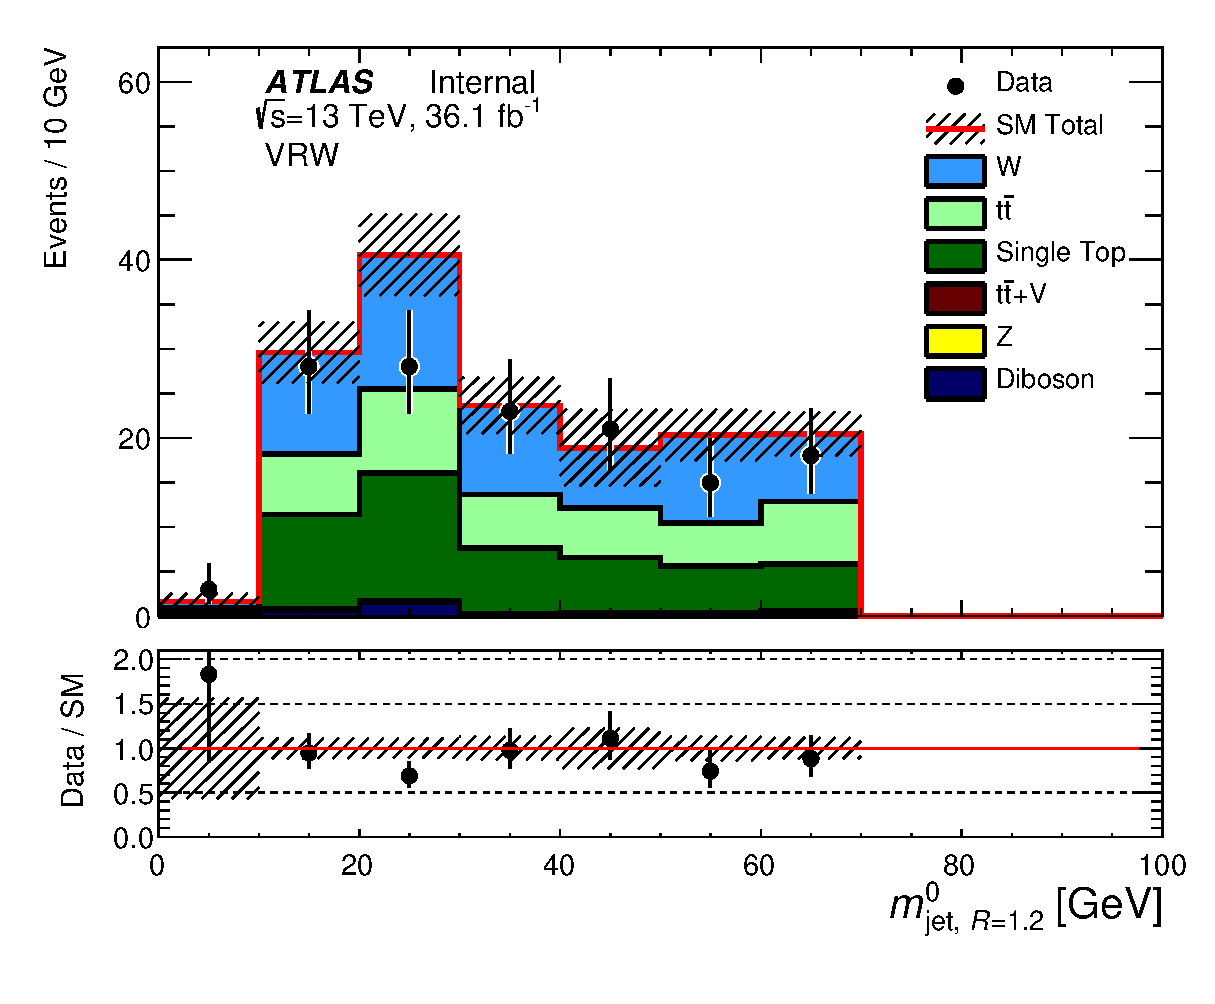
\includegraphics[width=0.45\textwidth]{figures/wJets/postfit/AntiKt12M_0__VRW.eps}
  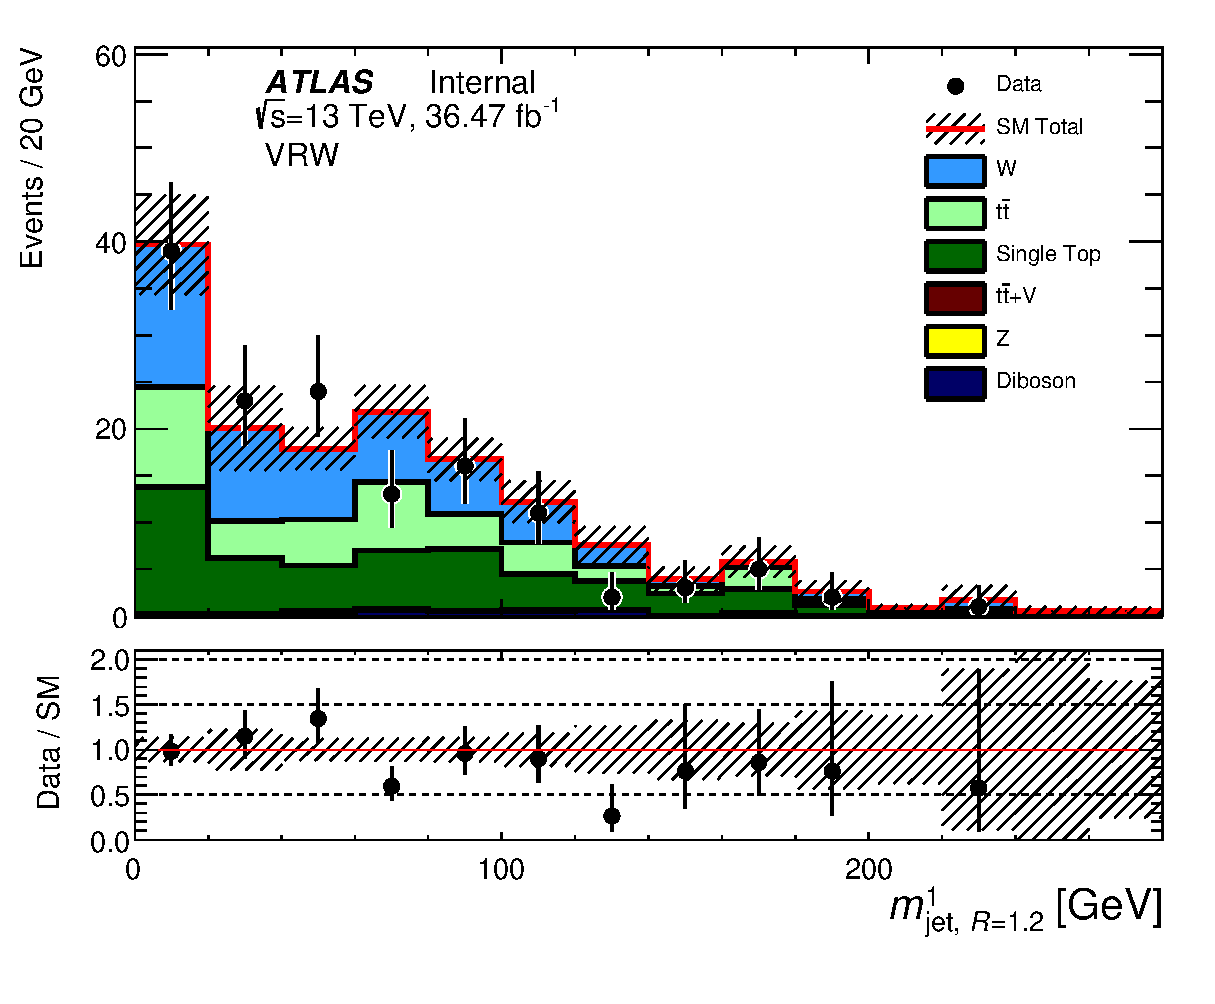
\includegraphics[width=0.45\textwidth]{figures/wJets/postfit/AntiKt12M_1__VRW.eps}
  \includegraphics[width=0.45\textwidth]{figures/wJets/postfit/AntiKt8M_0__VRW.eps}
  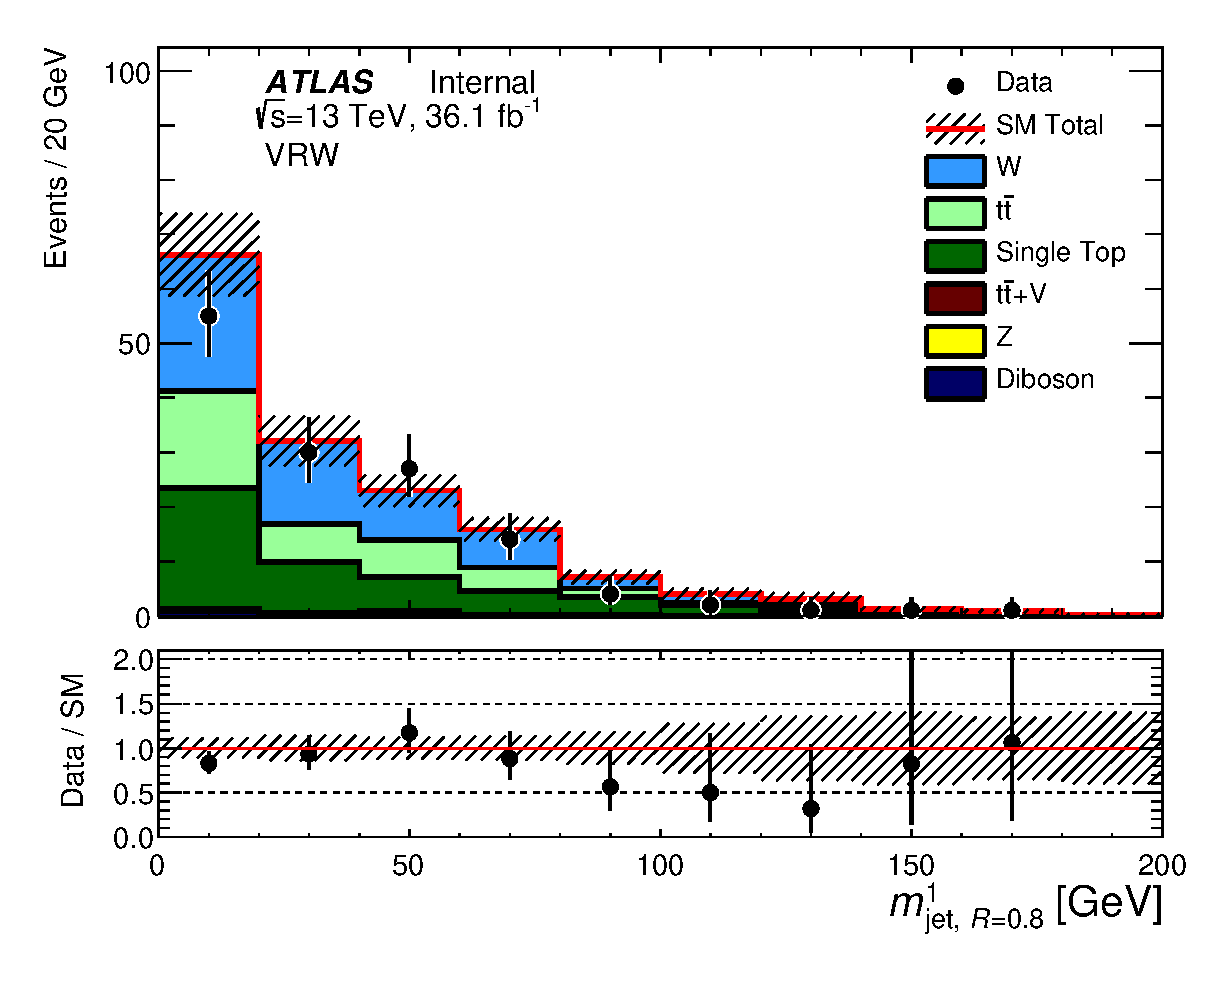
\includegraphics[width=0.45\textwidth]{figures/wJets/postfit/AntiKt8M_1__VRW.eps}
  \caption{Postfit data/MC comparisons in the VRW. From left to right and top to bottom, the variables shown are \met, \mtbmin, \mtbmax, \mantikttwelvezero, \mantikttwelveone, and \mantikteightzero. The background contributions from MC are normalised to \intlumi\ \ifb, and summed together, the data points are shown in black. The hatched band in the ratio shows the MC statistical and detecotor uncertainties.}
  \label{fig:VRWMasses}
\end{figure}


The relative \Wjets\ composition split in contributions from the CVetoBVeto, CFilterBVeto and BFilter samples in the \Wjets\ control region is 19.6\%, 36.6\%, and 43.7\% respectively. The same fractions in the WVR are 2.1\%, 7.7\%, and 90.2\%. As an example in SRB-T0 the \Wjets\ relative composition is 0.1\% CVetoBVeto, 11.8\% CFilterBVeto, 88.1\% BFilter - the numbers of CVetoBVeto and CFilterBVeto events in the SR are affected by very large uncertainty due to MC statistics. This shows that even though the composition in the CR does not reflect completely the SR composition, the VR is designed to have very similar type of events as the SR and being hence a very good test of the goodness of the Fit in the CR.

The $W+c$ contribution in the CR amounts to 9.73\%, in the VR to 5.15\%, and in SRC-high to 1.86\% (number based on 20.1, Sherpa 2.1 samples).

%% W CR (\intlumi\ ifb):
%% CVetoBVeto: 28.7183048946 +/- 2.8169946951
%% CFilterBVeto: 49.9653279331 +/- 3.09807868142
%% BFilter: 62.7871569086 +/- 1.90972859172

%% W VR (\intlumi\ ifb): 
%% CVetoBVeto: 0.437729296812 +/- 0.247392389588
%% CFilterBVeto: 2.24301148651 +/- 0.505270804979
%% BFilter: 17.247621849 +/- 0.852912878737

%% SRC-high (10 ifB):
%% CVetoBVeto: 0.00892772898078 +/- 0.00892772879617
%% CFilterBVeto: 0.253932834836 +/- 0.161437072511
%% BFilter: 1.18994702236 +/- 0.221031665671

%% For the (W+c)/(W+all) fractions, I can give you at the moment only the fractions from our old samples (20.1 and Sherpa 2.1), since that information is not in the Trees and our 20.7 samples are not yet finished, so the fraction might not be completely accurate (but should probably be not too bad):

%% W CR: 9.73%
%% W VR: 5.15%
%% SRC-high: 1.86%


\clearpage

